\section{Introduction}
This chapter presents the proposed methodology in full. The system is a two-stage computer-vision pipeline: a single-class detector localizes the waste item, and the cropped object is passed to a shared-backbone convolutional network with four task heads that jointly predict material, condition, disposal route, and an ordinal threat level. The heads are fused by a regulation-grounded decision layer with a safety backstop. The chapter describes, in order, the overall system (Section~\ref{sec:overview}), the experimental setup, the methodology workflow, the development of the dataset and every preprocessing operation applied to it, the detection stage and the detector architecture, the proposed multi-task network and its backbone, the loss functions, the training procedure, calibration, the decision layer, and the evaluation protocol. Each processing step is described together with the concrete operation that implements it, and every figure is described at the point where it is introduced.

\section{System Overview}
\label{sec:overview}
At inference time the system transforms one or more photographs of an item into an explainable disposal decision through the sequence shown in Figure~\ref{fig:System_Overview}. Each photograph is first localized by the detector and cropped to the item; the crop is colour-normalized and resized; a single backbone encodes it into a feature vector that feeds four task heads; the per-view head outputs are aggregated to the item; and a decision layer combines them into a final route, a reconciled threat level, a confidence value, and a human-readable explanation. The design includes validation-fitted temperature scaling before the decision layer. Calibration is evaluated separately on the three-backbone ensemble; the paired end-to-end crop comparison uses unscaled outputs.

\begin{figure}[!ht]
    \centering
    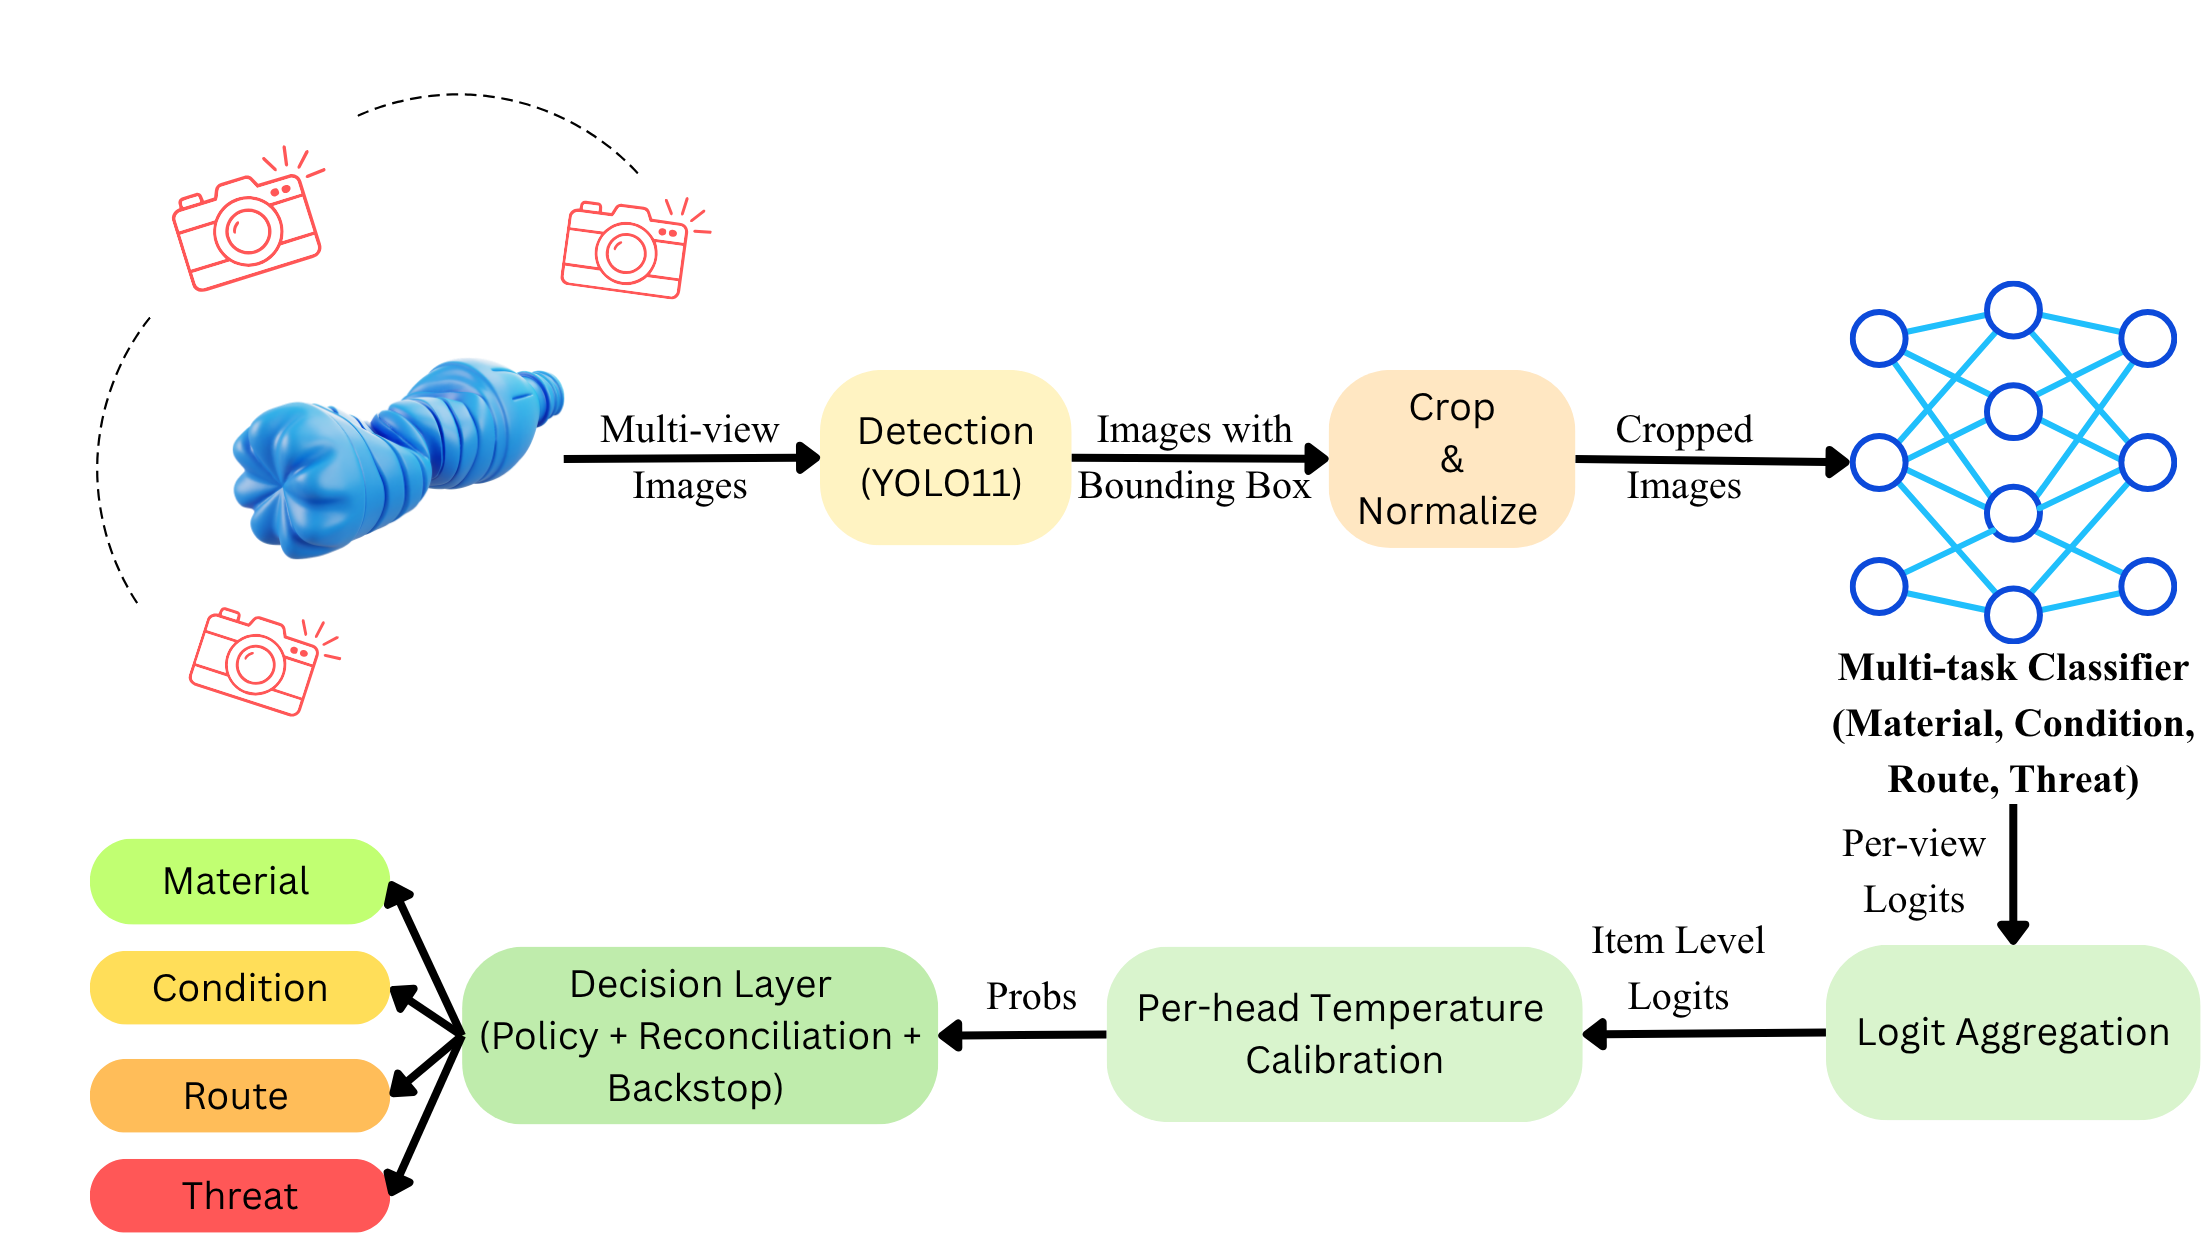
\includegraphics[width=\textwidth]{./figures/End_to_End_Inference.png}
    \caption{End-to-end inference pipeline of the proposed system.}
    \label{fig:System_Overview}
\end{figure}

Reading Figure~\ref{fig:System_Overview} along its data flow: the input photograph passes through the YOLO11 detector, which returns the highest-confidence bounding box; the box is cropped and sent through the preprocessing chain (gray-world white balance, resize to $224\times224$, ImageNet normalization); the ConvNeXt-S backbone encodes the crop into a $768$-dimensional feature that fans out to the four task heads; the per-view logits are averaged into item-level logits, with a per-head temperature-calibration stage in the design; and the decision layer finally combines them into the routing decision, threat level, confidence, and explanation. The rationale for the two-stage design is that localizing the object first reduces background clutter and focuses classification on the item. A single shared backbone feeding four lightweight heads is parameter-efficient, because the related tasks learn from one common representation.

Whereas Figure~\ref{fig:System_Overview} presents the pipeline as a single linear data flow, Figure~\ref{fig:Flowchart} renders the same system as a control-flow flowchart in which the decision logic and its branches are made explicit, so that the safety-critical routing behaviour can be traced from input to output.

\begin{figure}[!ht]
    \centering
    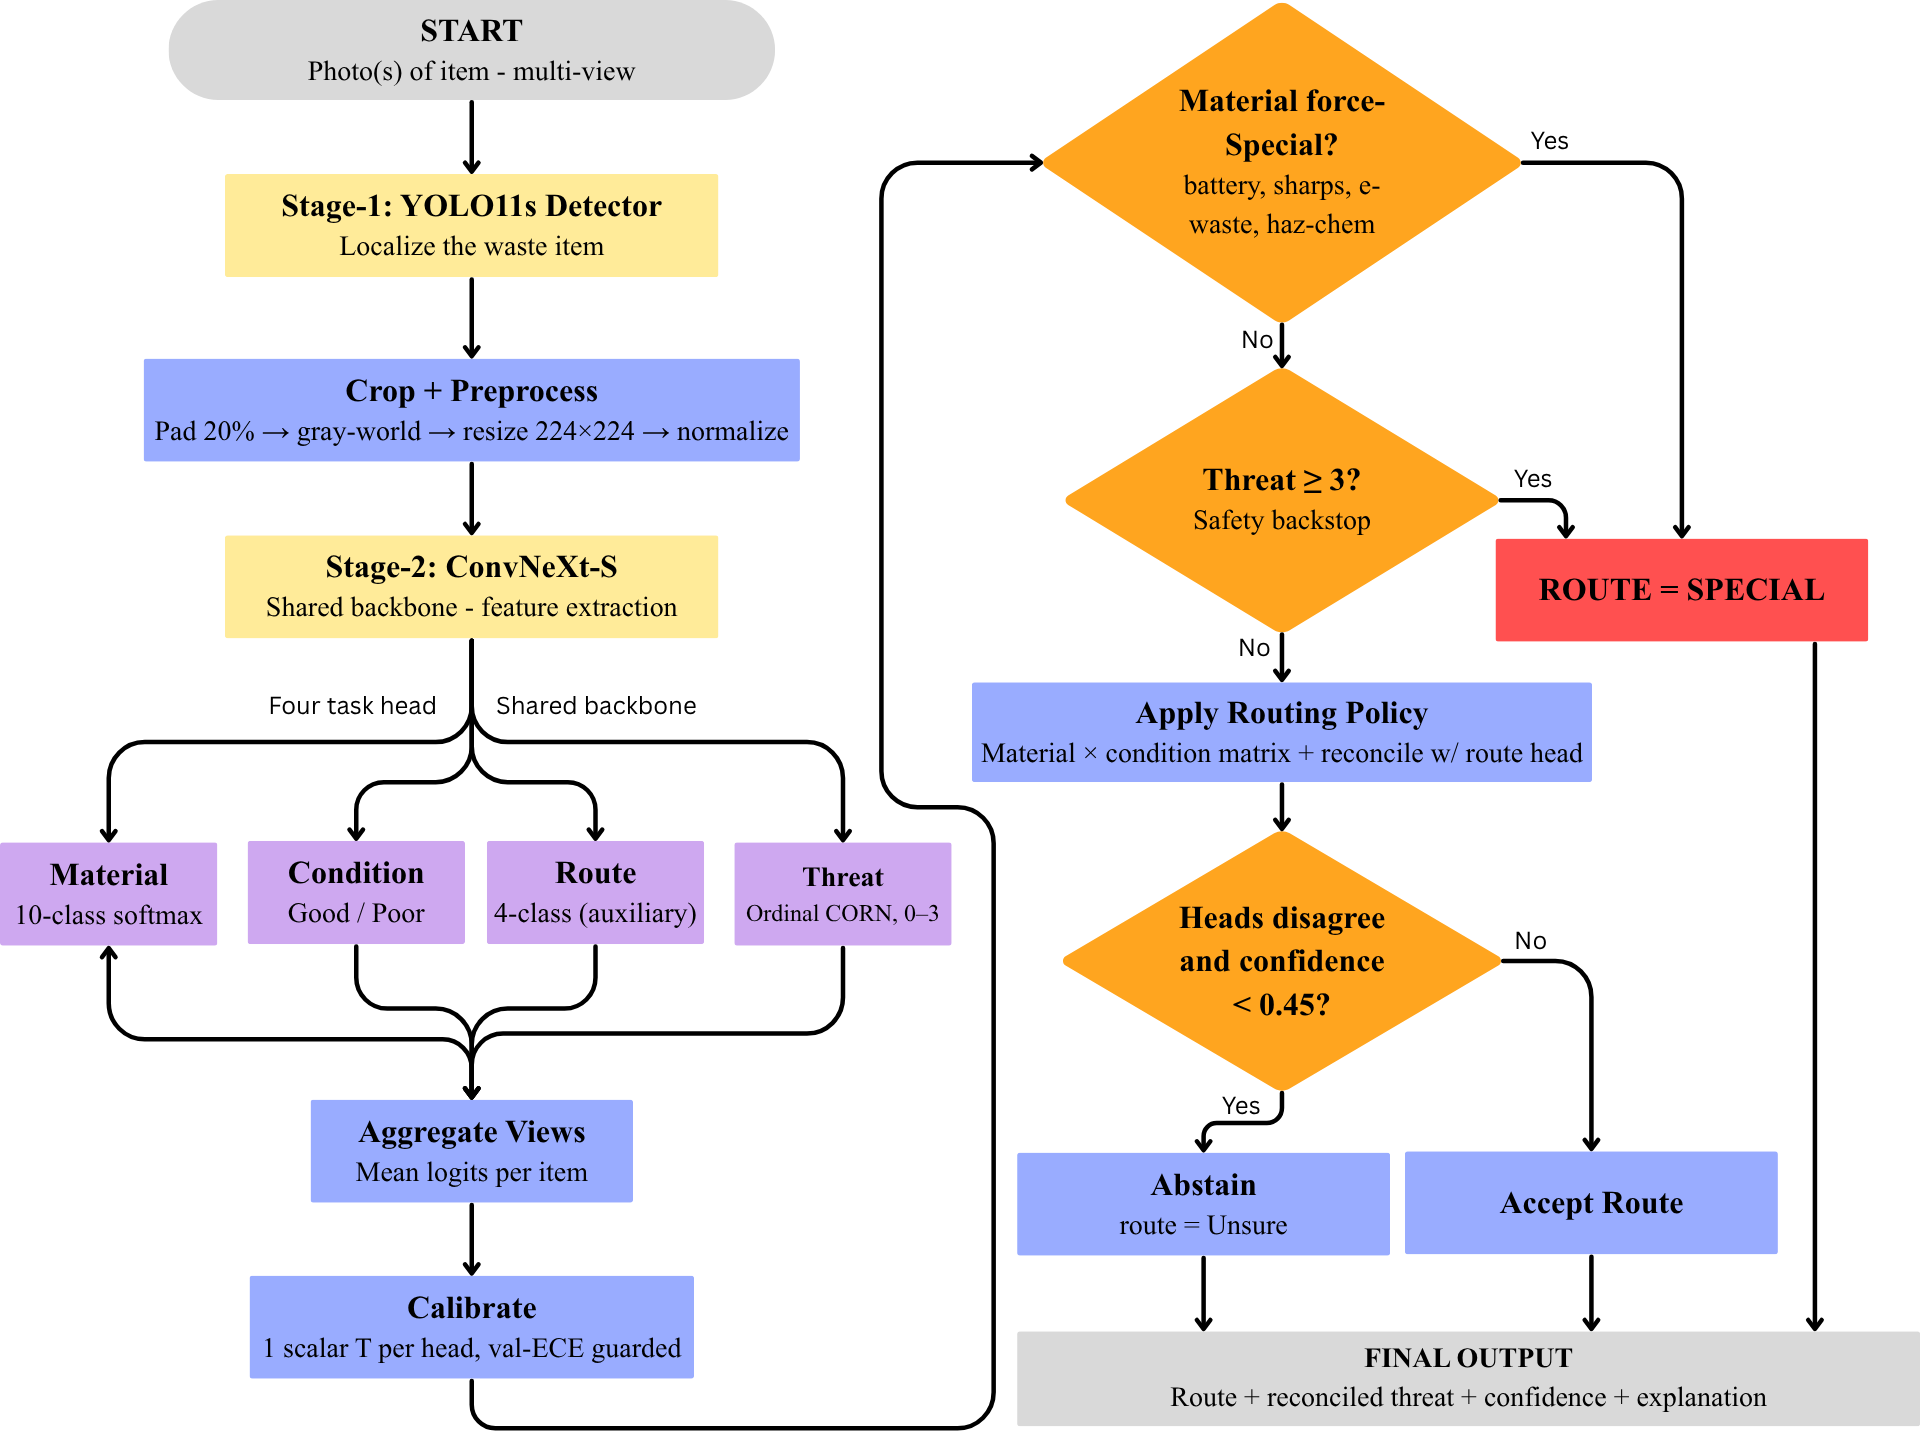
\includegraphics[width=\textwidth]{./figures/Flow_Chart.png}
    \caption{Working-process flowchart of the complete system, from the input photograph to the final routing decision, exposing the decision-layer branches and the threat-aware safety backstop.}
    \label{fig:Flowchart}
\end{figure}

Reading Figure~\ref{fig:Flowchart} from the top left, photographs of the item enter the Stage-1 YOLO11s detector, which localizes the waste object; the crop is preprocessed (a $20\%$ expansion of the box's longer side, gray-world white balance, resize to $224\times224$, and ImageNet normalization) and encoded by the Stage-2 ConvNeXt-S shared backbone, whose feature fans out to the four task heads (material, condition, route, and threat). The flowchart shows item-level averaging followed by per-head temperature calibration, and control then passes to the decision cascade in the right-hand column. That cascade is a priority-ordered sequence of tests in which the first match wins: if the predicted material is one of the force-Special streams (battery, sharps, e\_waste, hazardous\_chemical) the route is set to Special at once; otherwise, if the reconciled threat level is $\ge 3$, the threat-aware safety backstop forces Special regardless of the material label; otherwise the material$\times$condition routing policy is applied and reconciled with the learned route head. A final abstention gate emits ``Unsure'' only when the heads disagree and material confidence is below $0.45$, while a Special decision is never abstained. Every branch converges on the final route, reconciled threat, decision confidence, and explanation. The two orange decision diamonds express the system's safety constraints; the detailed rules are given in the Decision Layer section (Figure~\ref{fig:Decision}).

\section{Experimental Setup}
All experiments were implemented in Python with PyTorch, using the timm library \cite{timm} for backbone architectures and pretrained weights and the Ultralytics package \cite{yolo11} for the detector. Training and evaluation were performed on cloud GPU notebooks (Kaggle). A fixed random seed (42) is used for data splitting and is set for Python, NumPy, and PyTorch in the training routine to support reproducibility of augmentation and sampling. The baseline classifiers share the same losses, seed, and item split; the larger and register-token transformers use the specialised fine-tuning procedure described below. Detector candidates are compared under a common training budget and split.

\section{Methodology Workflow}
The development workflow, from raw data to a validated system, is summarized in Figure~\ref{fig:Architecture}. Data are prepared once; the candidate backbones are then trained under the baseline or specialised transformer recipe; the detector is trained separately on the same items; calibration is fitted on the validation split; the decision layer is assembled; and the system is finally evaluated under several protocols.

\begin{figure}[!ht]
    \centering
    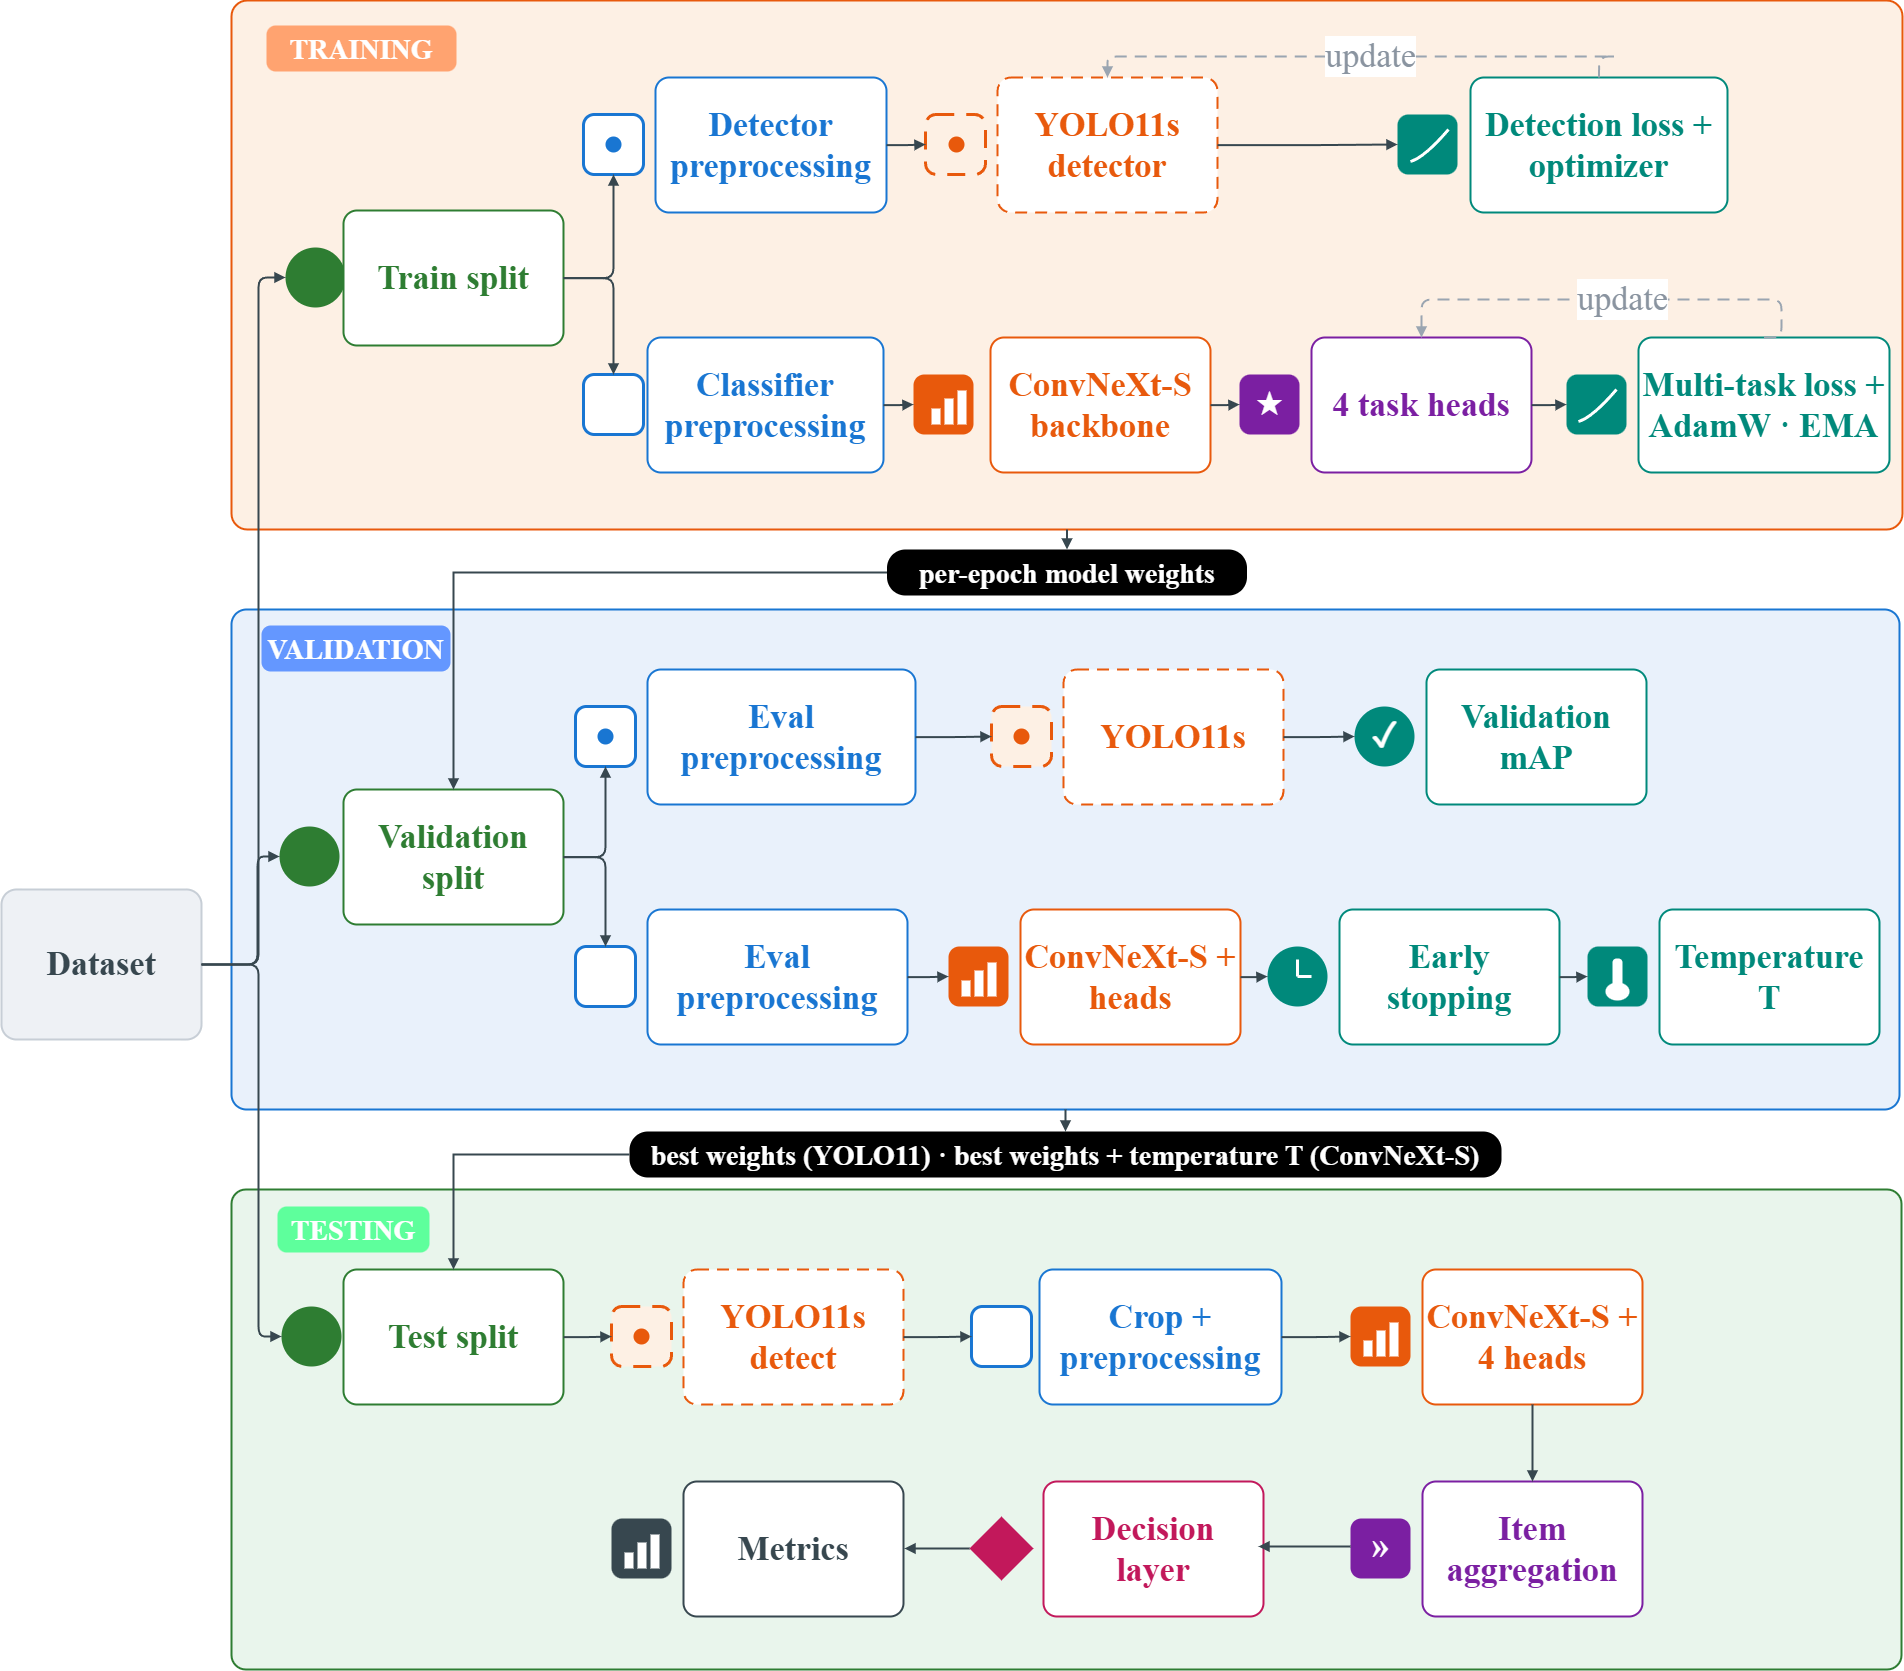
\includegraphics[
        width=\textwidth,
        height=.57\textheight
    ]{./figures/pipeline_architecture.png}
    \caption{Training, validation, and testing workflow of the two-stage system.}
    \label{fig:Architecture}
\end{figure}

Figure~\ref{fig:Architecture} is organized as three coloured phase bands. In the training band the item-level train split feeds two parallel lanes: the YOLO11 detector, trained with box, class, and distribution-focal losses, and the ConvNeXt-S backbone with four heads, trained with focal, binary cross-entropy, label-smoothed cross-entropy, and CORN losses under AdamW with an exponential moving average of the weights. In the validation band the per-epoch weights are evaluated: the detector by validation mAP for best-checkpoint selection, and the classifier by the composite early-stopping score followed by per-head temperature calibration. In the testing band the models are chained end-to-end (detect, crop, classify, aggregate views, decide) and the final metrics are computed; the connectors between bands carry the per-epoch weights downward and show the best weights plus fitted temperatures entering a calibrated test. Training and validation use ground-truth classifier crops, while the end-to-end test uses predicted boxes. An additional oracle-crop test uses ground-truth boxes to quantify the localization cost separately. Model selection uses a task-weighted composite score, and calibration is fitted on validation data.

\section{Dataset Development}
The dataset was purpose-built to capture waste under varied real-world conditions and to carry the four annotations the system predicts. Figure~\ref{fig:datasetdev} shows the development flow, whose substeps are described below.

\begin{figure}[!ht]
    \centering
    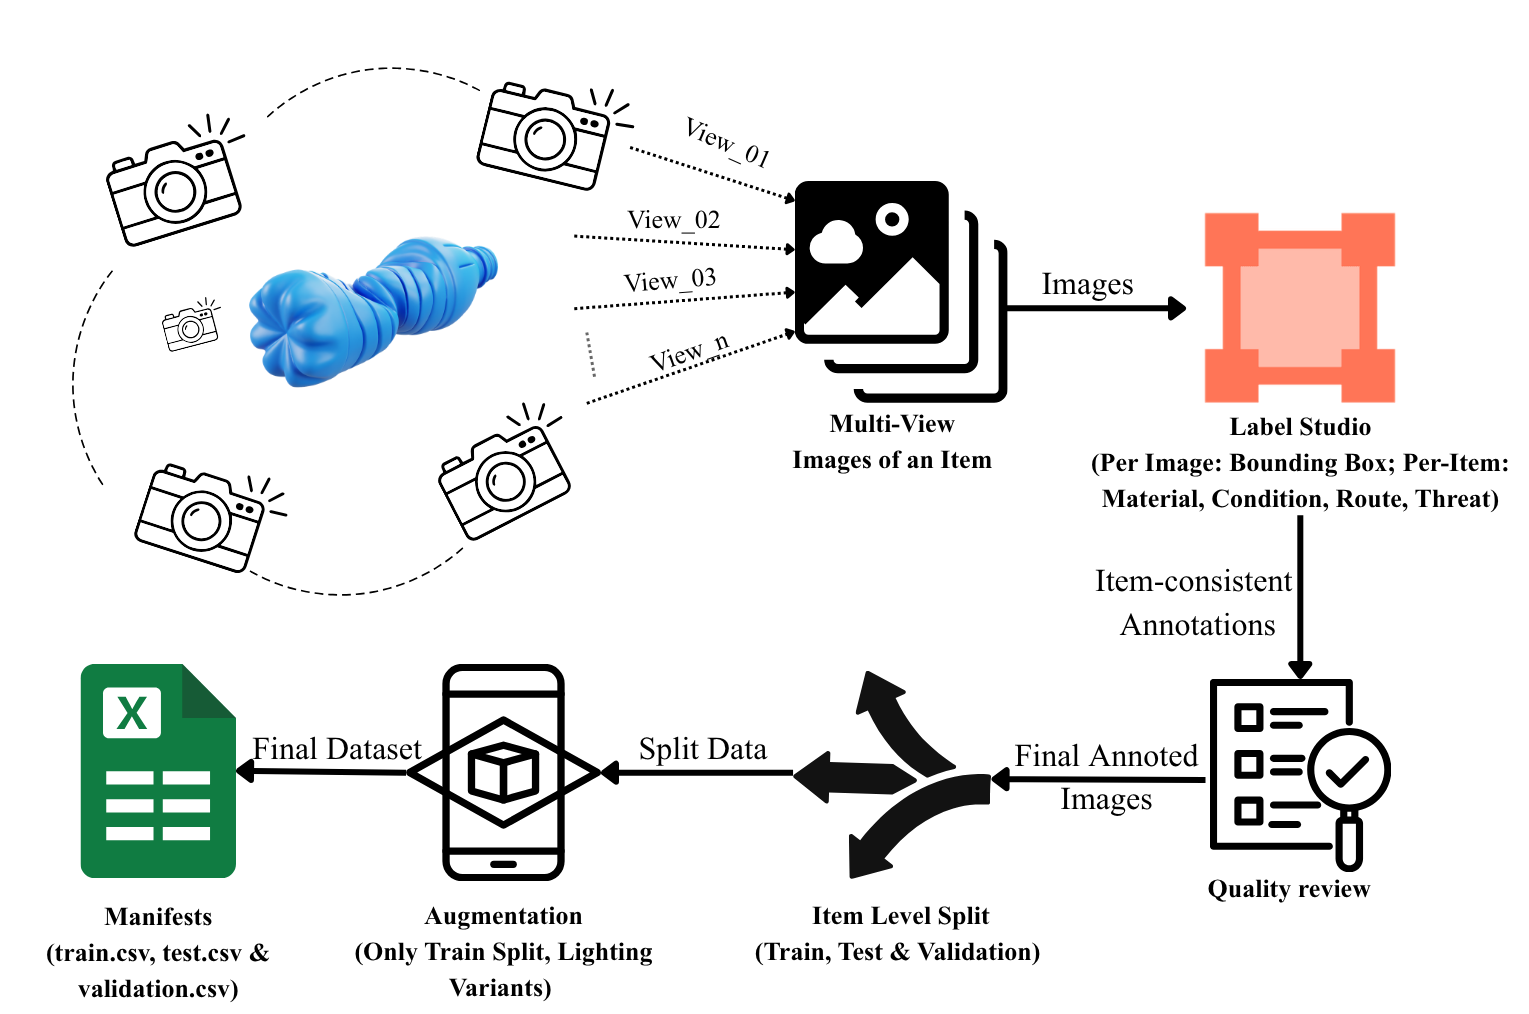
\includegraphics[width=\textwidth]{./figures/Dataset_Development.png}
    \caption{Dataset development flow from acquisition to leakage-checked splits.}
    \label{fig:datasetdev}
\end{figure}

Figure~\ref{fig:datasetdev} traces the data from physical acquisition to the leakage-controlled manifests that the rest of the pipeline consumes: physical items are catalogued and photographed from multiple views under varied lighting and background; each item is annotated with a bounding box and the four labels; the annotated views are split by item into train, validation, and test manifests; and a leakage check confirms that no item crosses splits. Each stage of the flow is detailed in the following subsections.

\subsection{Acquisition}
The dataset comprises 485 waste items photographed under varied real-world conditions, with 5{,}363 image entries across the training, validation, and test manifests (4{,}926, 216, and 221, respectively), including augmented training images. Lighting, background, viewing angle, and physical wear vary across the images. The physical item, not the image, is the unit of classifier and decision analysis; its several photographs are treated as different views of the same object, and classification metrics are computed after aggregating an item's views. This item-centric design mirrors the real task, in which a single decision must be made about one physical object seen from the available angles.

\subsection{Labelling Scheme}
Every item is annotated along four dimensions and with an object bounding box. The label spaces are listed in Table~\ref{tab:labels} and visualized in Figure~\ref{fig:Labelling_Scheme}.

\begin{figure}[!ht]
    \centering
    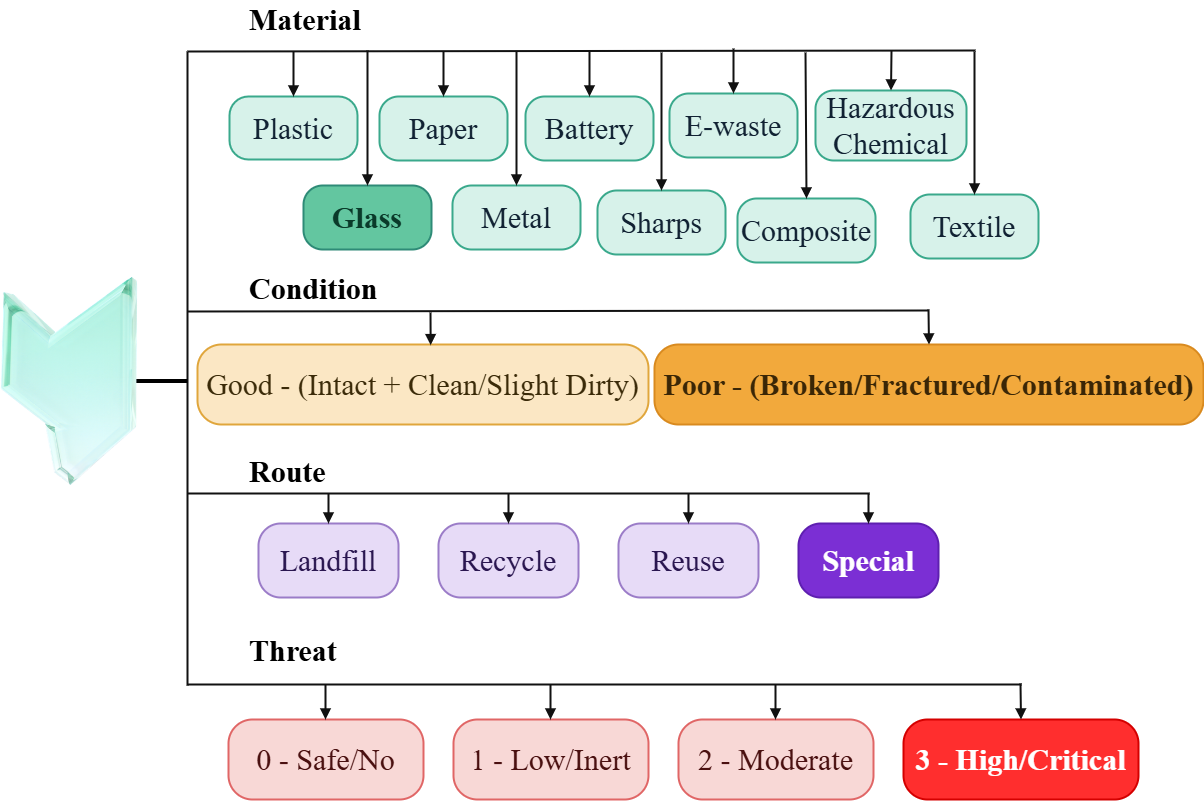
\includegraphics[height=9cm,width=\textwidth]{./figures/Labelling_Scheme.png}
    \caption{Labelling scheme: the four annotation dimensions of every item.}
    \label{fig:Labelling_Scheme}
\end{figure}

Figure~\ref{fig:Labelling_Scheme} makes the multi-task structure explicit: a single waste item carries four simultaneous annotations, a ten-way material class, a binary condition (Good or Poor), a four-way route (Reuse, Recycle, Landfill, Special), and an ordinal threat level. Good denotes an intact item that is clean or slightly dirty, whereas Poor covers broken, fractured, or contaminated items. Threat is drawn as a graded scale to emphasize that its levels are ordered rather than nominal. The four heads share one input crop but predict distinct, partly dependent label spaces, which is why each head is paired with a task-appropriate loss; the CORN ordinal loss exploits the threat ordering.

A concrete application of this scheme to a single real item is shown in Figure~\ref{fig:labelling_example}. Item~106 is a piece of broken glass photographed from several angles; one representative view carries the object bounding box tagged with the material class glass, and the two smaller views show the same physical object from other angles. All three views share a single item-level label set: material glass, condition Poor, disposal route Special, and threat level~3. The example makes the item-centric design concrete and exposes the material--condition dependency encoded by the routing policy: glass in Poor condition is escalated to Special and the maximum threat level.

\begin{figure}[!ht]
    \centering
    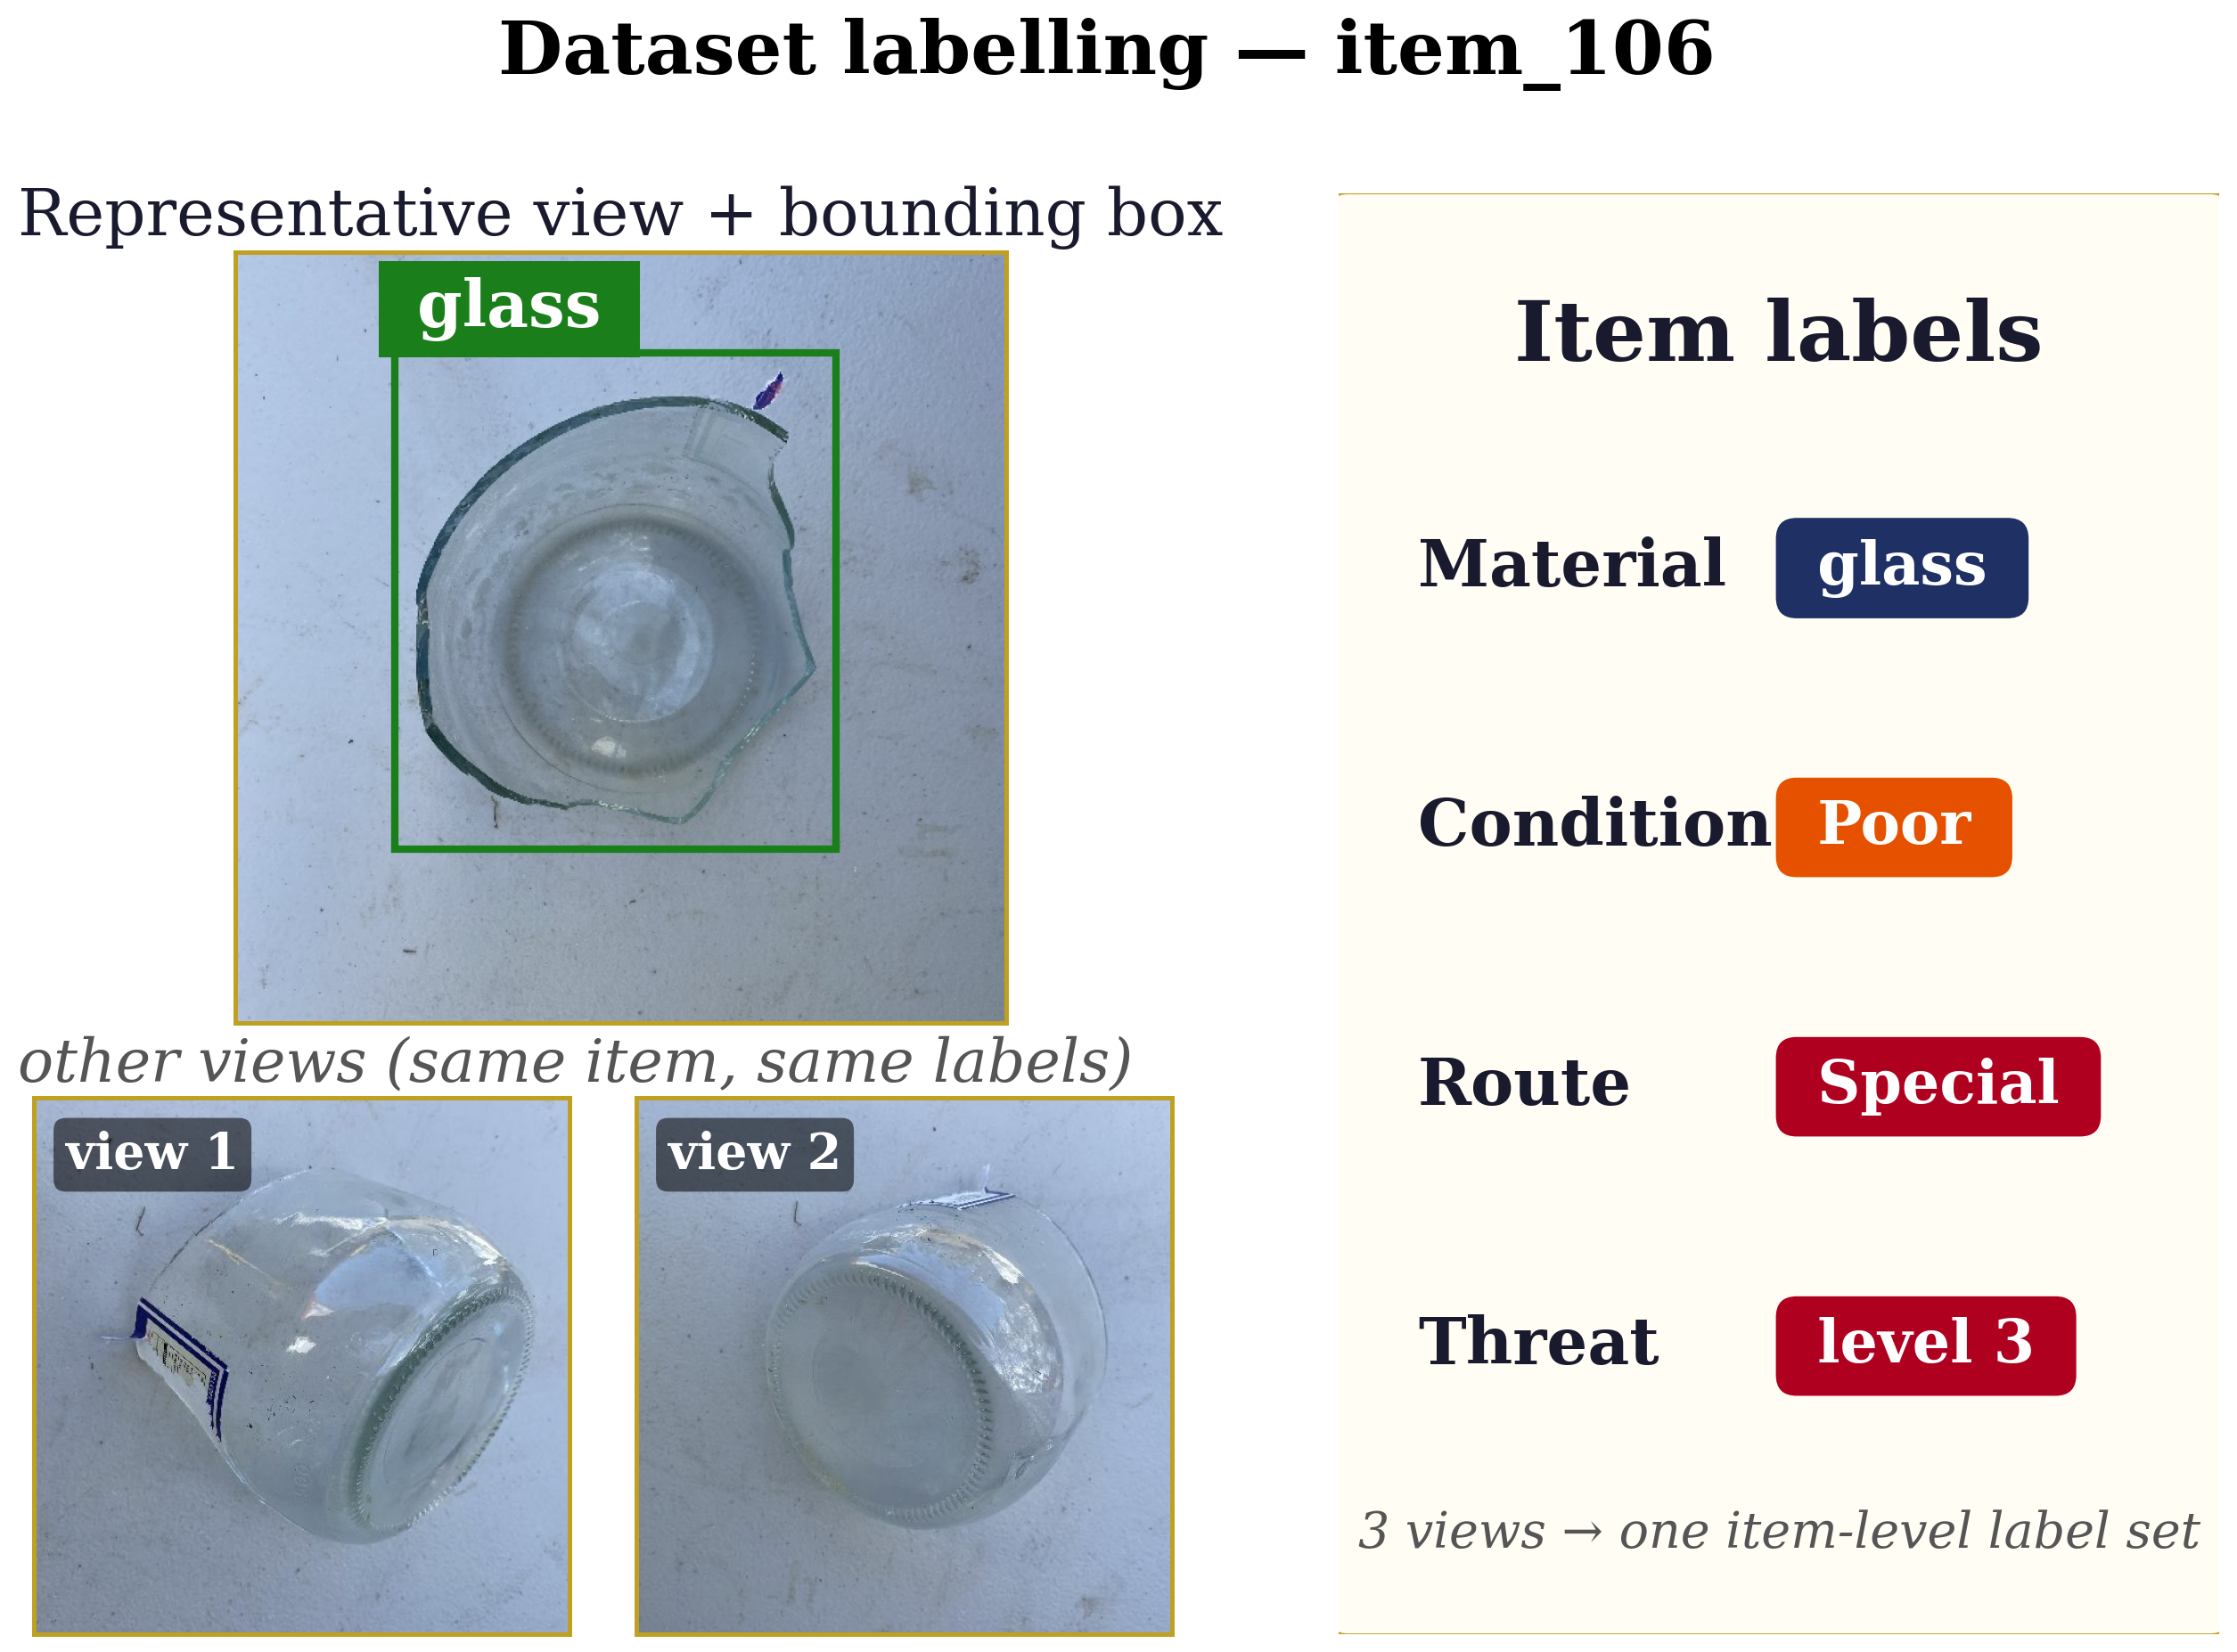
\includegraphics[height=7cm,width=\textwidth]{./figures/fig1_labelling_transparent.png}
    \caption{The labelling scheme applied to one real item (item~106, broken glass).}
    \label{fig:labelling_example}
\end{figure}

\begin{table}[!ht]
\centering
\caption{Label spaces of the four prediction tasks.}
\label{tab:labels}
\begin{tabularx}{\linewidth}{@{}l Y@{}}
\toprule
\textbf{Dimension} & \textbf{Classes} \\
\midrule
Material (10) & plastic, paper, metal, glass, textile, e\_waste, battery, sharps, hazardous\_chemical, composite \\
\addlinespace[3pt]
Condition (2) & Good, Poor \\
\addlinespace[3pt]
Route (4) & Reuse, Recycle, Landfill, Special \\
\addlinespace[3pt]
Threat (ordinal) & Litter Impact Index level 0, 1, 2, 3 \\
\bottomrule
\end{tabularx}
\end{table}

\textbf{Threat scale.} Threat is annotated on the Litter Impact Index (LII) \cite{lii}, an ordered scale from 0 (no harm) to 3 (direct human harm), defined in Table~\ref{tab:threat}. The dataset contains 130 level-1, 194 level-2, and 161 level-3 items, with no level-0 samples. The $0$--$3$ range is retained for fidelity to the LII and is represented by three conditional CORN outputs; the observed threat labels occupy levels 1--3.

\begin{table}[!ht]
\centering
\caption{Threat severity (Litter Impact Index) \cite{lii}.}
\label{tab:threat}
\begin{tabularx}{\linewidth}{@{}c l Y@{}}
\toprule
\textbf{LII} & \textbf{Definition} & \textbf{Exemplars in this taxonomy} \\
\midrule
0 & No harm (inert/safe) & reserved, no samples in dataset \\
1 & Indirect harm (litter) & paper, metal, textile \\
2 & Wildlife entanglement / ingestion & plastic, intact glass, composite \\
3 & Direct human harm & broken glass, sharps, e\_waste, battery, hazardous\_chemical \\
\bottomrule
\end{tabularx}
\end{table}

\textbf{Routing rules.} Routing follows a Bangladesh-first regulatory basis (Solid Waste Management Rules 2021 \cite{bdswm2021}; National 3R Strategy \cite{bd3r2010}) with a hazardous ``Special'' safety overlay drawn from international standards (US EPA Universal Waste \cite{epauw}, EU WEEE \cite{weee}, OSHA \cite{osha}, WHO \cite{who}, CDC \cite{cdc}) and Bangladesh hazardous, e-waste, and medical-waste rules \cite{bdhazardous2011,bdewaste2021}. The deterministic routing matrix is given in Table~\ref{tab:routing}.

\begin{table}[!ht]
\centering
\caption{Routing matrix: material $\times$ condition $\rightarrow$ route.}
\label{tab:routing}
\begin{tabular}{lcccc}
\toprule
\textbf{Material} & \textbf{Good} & \textbf{Poor} & \textbf{Threat} & \textbf{Force-Special} \\
\midrule
plastic & Recycle & Landfill & 2 & No \\
paper & Recycle & Landfill & 1 & No \\
metal & Recycle & Recycle & 1 & No \\
glass & Recycle & Special & 2 & via condition \\
textile & Reuse & Recycle & 1 & No \\
e\_waste & Special & Special & 3 & Yes \\
battery & Special & Special & 3 & Yes \\
sharps & Special & Special & 3 & Yes \\
hazardous\_chemical & Special & Special & 3 & Yes \\
composite & Landfill & Landfill & 2 & if hazardous sub-part \\
\bottomrule
\end{tabular}
\end{table}

The threat column in Table~\ref{tab:routing} gives the material prior; glass in Poor condition raises this prior from 2 to 3. For a predicted composite, a force-Special material among the top two material probabilities with probability above $0.15$ activates the hazardous-sub-part rule.

\subsection{Preprocessing}
Each image passes through a fixed preprocessing chain before it reaches the network, implemented in the dataset's item reader (WasteDataset) and shown in Figure~\ref{fig:Preprocessing}.

\begin{figure}[!ht]
    \centering
    
\includegraphics[width=0.8\textwidth]{./figures/Preprocessing.png}
    \caption{Classifier preprocessing chain.}
    \label{fig:Preprocessing}
\end{figure}

In Figure~\ref{fig:Preprocessing} the raw RGB image and its bounding box enter at the top; the item is cropped with a small padding margin, gray-world white balancing suppresses colour casts introduced by varied lighting, the crop is resized to $224\times224$, a train-only augmentation branch applies horizontal flip, mild rotation, colour jitter, blur, and coarse dropout, and ImageNet channel normalization finally produces the tensor fed to the backbone. The chain corresponds to the following operations:
\begin{enumerate}
    \item load\_rgb reads the image as an RGB array with EXIF orientation applied.
    \item object\_crop crops to a square centred on the annotated box with side length $1.2\max(w,h)$, providing a $20\%$ expansion while retaining context. The crop is clipped to the image boundaries, and a centre square crop is used when no valid box is available.
    \item gray\_world applies a gray-world white balance, scaling the colour channels to a common mean to suppress the colour casts introduced by varied lighting, which is important because material appearance is colour-sensitive.
    \item apply\_tf resizes the crop to $224\times224$ and converts it to a normalized tensor using the ImageNet channel statistics; for the training split it applies the augmentation transform train\_tf, and for validation and test the deterministic eval\_tf.
\end{enumerate}
The detector uses a separate preprocessing path (letterbox resize to $640\times640$ and pixel scaling to $[0,1]$, with mosaic and colour augmentation at training time); the two paths share only the raw-image load and diverge immediately, because the detector operates on the full frame while the classifier operates on the crop.

Figure~\ref{fig:preprocessing_example} shows both paths applied to the same real item, item~106, making the shared-input-then-diverge structure explicit. The detector path (top) letterboxes the full frame to $640\times640$ and scales pixels to $[0,1]$ before the YOLO11 detector; the classifier path (bottom) crops the item with a $20\%$ side-length expansion, applies gray-world white balance, resizes to $224\times224$, and applies ImageNet normalization before ConvNeXt-S. The dashed panels illustrate train-time augmentation: mosaic and colour jitter for the detector, and horizontal flip, colour jitter, and coarse dropout for the classifier. They show augmentation examples; pixel-space classifier augmentation precedes normalization and applies only to training. Validation and test use deterministic preprocessing and the evaluation-time averaging described below.

\begin{figure}[!ht]
    \centering
    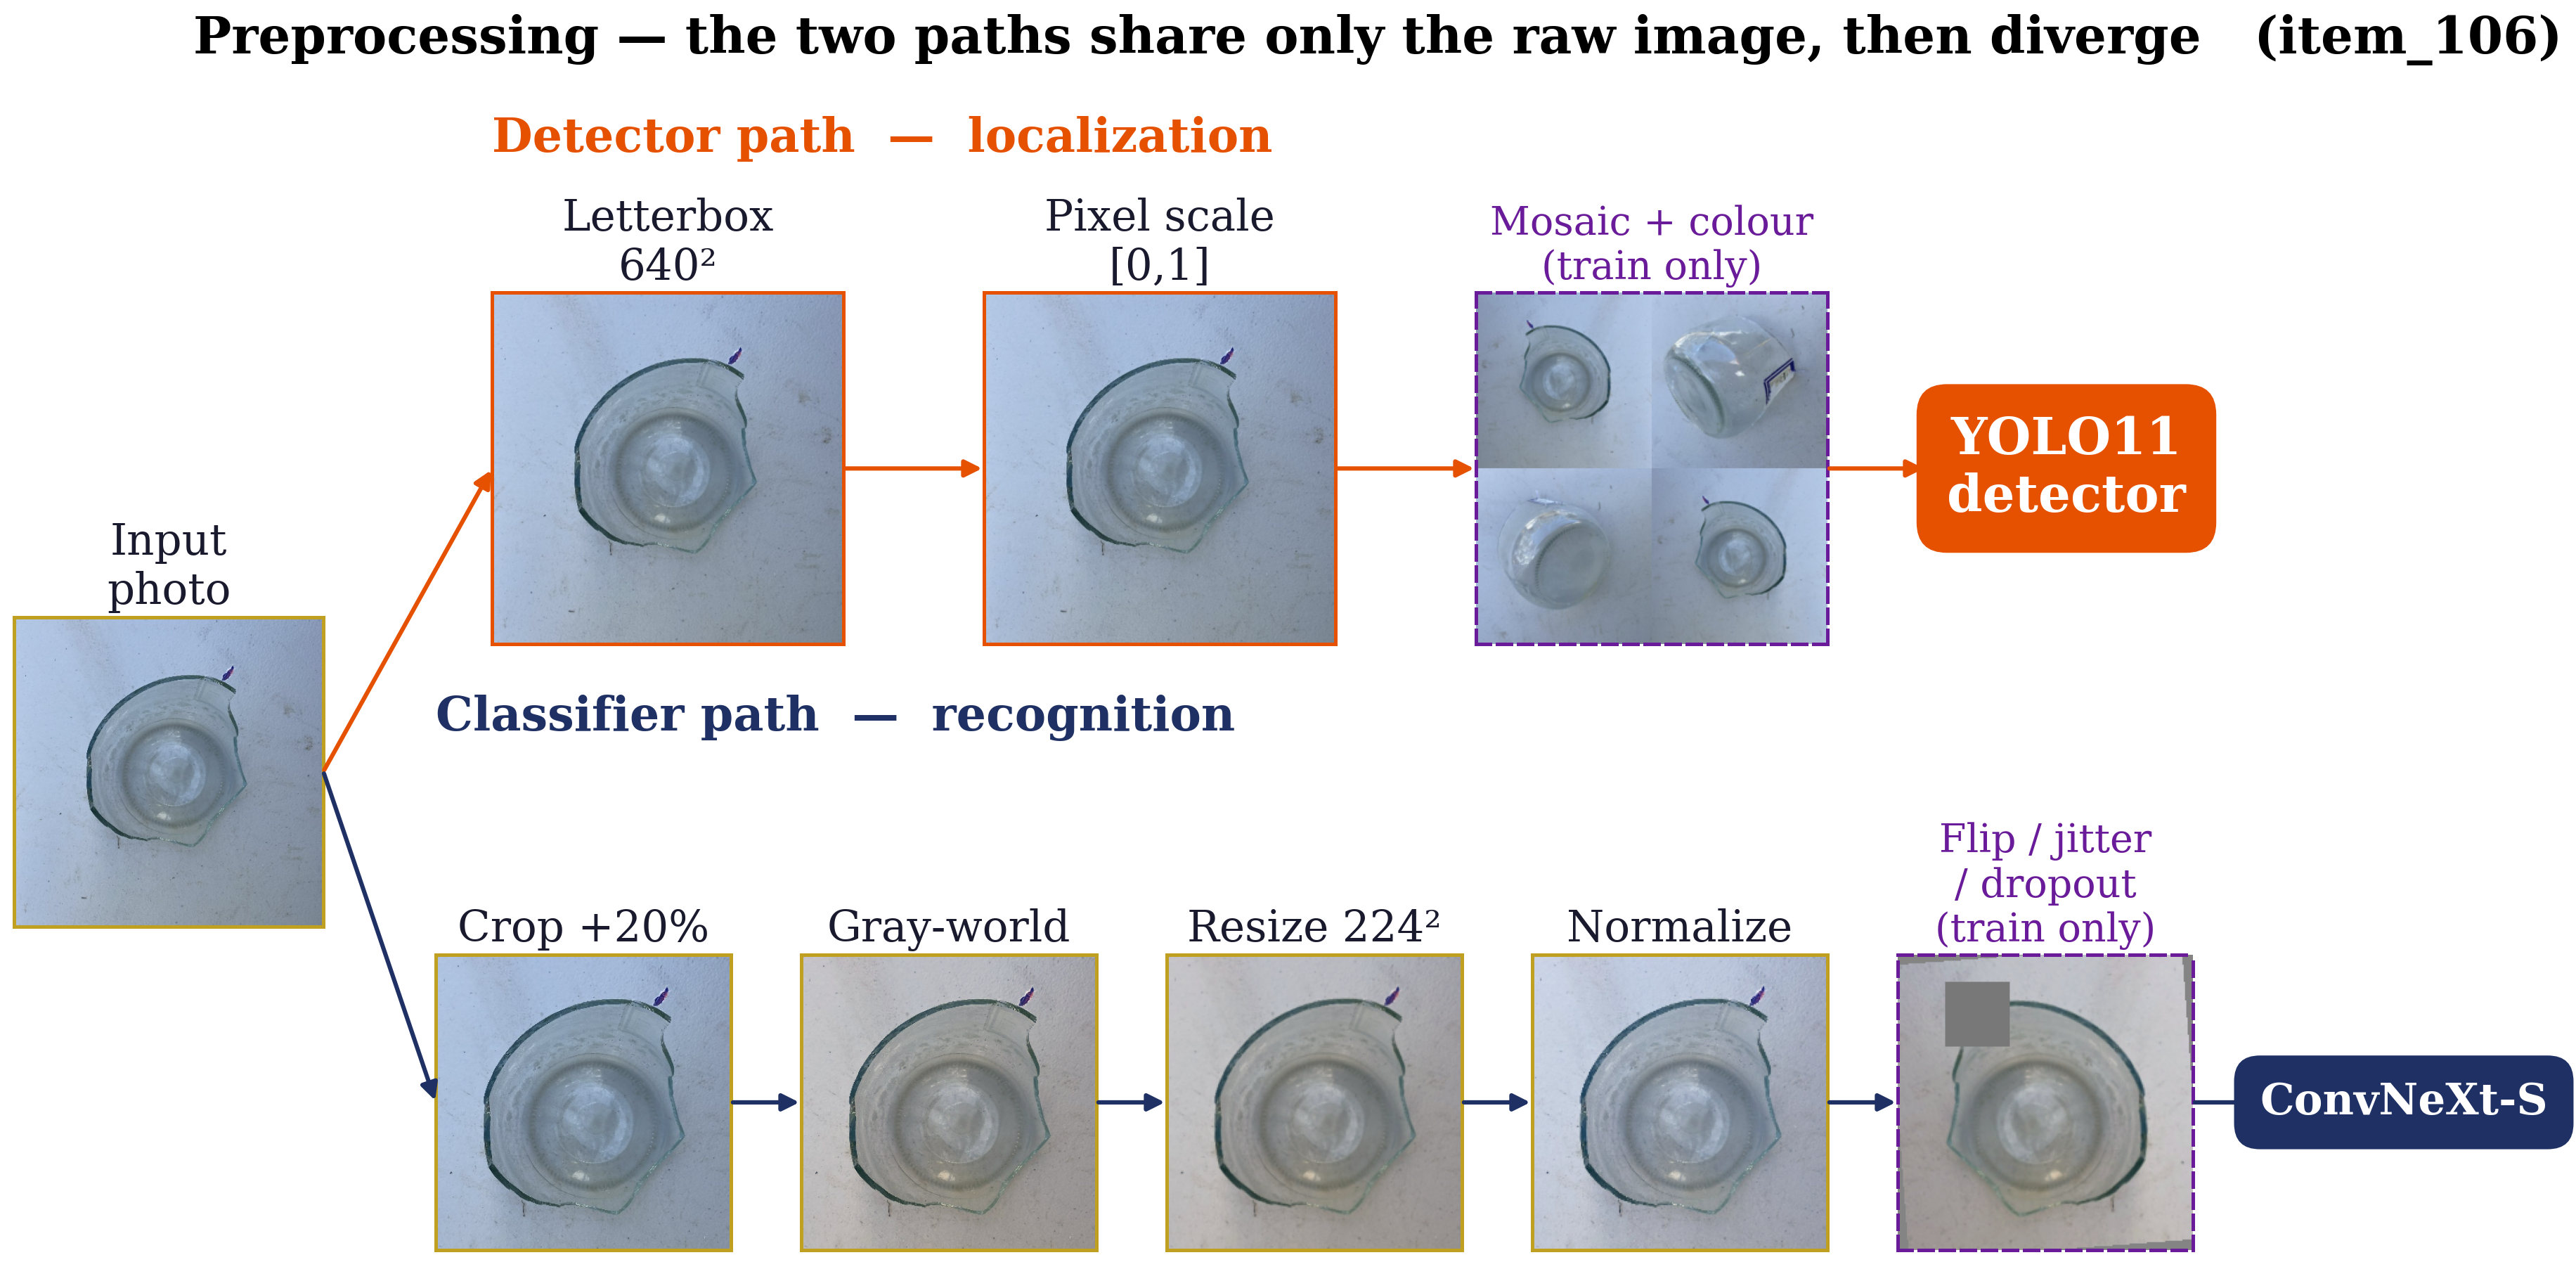
\includegraphics[height=6cm,width=.9\textwidth]{./figures/fig2_preprocessing_transparent.png}
    \caption{Both preprocessing paths applied to one real item (item~106).}
    \label{fig:preprocessing_example}
\end{figure}

\subsection{Augmentation and Class Balancing}
Augmentation (horizontal flips, mild rotations and colour perturbation, blur, and coarse dropout, in train\_tf) is applied to the training split only; validation and test use deterministic transforms. To counter class imbalance during training, the data loader draws samples with a WeightedRandomSampler built by make\_sampler, which assigns each image entry a sampling weight inversely proportional to its material-class frequency and samples with replacement, so rare classes appear more often per epoch.

\subsection{Item-Level Split and Manifests}
The dataset is split by item into 385 training, 50 validation, and 50 test items, so that all views of a given item, and any augmented copies, remain within a single split. A dedicated check (check\_leakage) verifies that no item identifier appears in more than one split. This item-level partitioning is essential: an image-level split would leak views of the same physical object across train and test and inflate measured performance. The split is recorded as training, validation, and test manifests that the rest of the pipeline consumes.

\subsection{Class Distribution}
The class distribution across materials, routes, and threat levels is shown in Figure~\ref{fig:dist}; the distribution is markedly imbalanced, with plastic containing 107 items and the smallest classes, textile and e\_waste, containing 26 and 30 items. Composite and hazardous\_chemical contain 34 and 36 items, respectively.

\begin{figure}[!ht]
    \centering
    \begin{subfigure}{0.49\textwidth}\centering\figorbox{figures/material_distribution.png}\caption{Ten material classes.}\label{fig:matdist}\end{subfigure}\hfill
    \begin{subfigure}{0.49\textwidth}\centering\figorbox{figures/route_threat_distribution.png}\caption{Routes and threat levels.}\label{fig:rtdist}\end{subfigure}
    \caption{Class distribution of the dataset across materials, disposal routes, and threat levels.}
    \label{fig:dist}
\end{figure}

In Figure~\ref{fig:matdist} the bars are sorted by frequency: common recyclables (plastic, glass, metal, paper) dominate, while textile and e\_waste form the smallest classes. Figure~\ref{fig:rtdist} shows the resulting route distribution (Reuse 14, Recycle 154, Landfill 133, Special 184) and threat distribution (levels 1, 2, and 3 with 130, 194, and 161 items). Each distribution totals 485 items.

\textbf{On the class imbalance.} The distributions in Figures~\ref{fig:matdist} and~\ref{fig:rtdist} reflect the material mix and collection conditions. The route and threat distributions reflect the annotated material mix and condition: Reuse is rare because only Good textile follows the reusable route, whereas Special is common because several material classes are force-routed there. Threat level 0 is absent from the annotated sample. The imbalance is addressed at the modelling level through class-weighted focal loss and inverse-frequency sampling for the material head and class-weighted cross-entropy for the route head (Table~\ref{tab:hyper}), and at the evaluation level through macro-F1, per-class scores, and item-level cross-validation.

\section{Detection Stage}
\label{sec:detection}
A single-class detector is trained to localize the waste item (one ``waste\_item'' class) from the per-item bounding-box annotations. At inference, detect\_\allowbreak top\_\allowbreak crop runs the detector, keeps the highest-confidence box, and crops it with crop\_from\_pred; if no box is returned this helper falls back to a centre crop. The paired crop evaluation instead provides a ground-truth fallback, which remained unused because every test view was detected. Localization focuses the classifier on the waste object.

\subsection{Detector Families Considered}
Two detector families are considered: single-stage YOLO detectors, which predict boxes densely in one forward pass, and transformer detectors of the DETR family, which pose detection as set prediction with attention. To choose the localizer, the members of both families summarized in Table~\ref{tab:det_families} were compared under a common training budget (60 epochs, $640\times640$ input, batch 16, the same item split and seed). The empirical comparison is reported in the Results chapter.

\begin{table}[!ht]
\centering
\caption{Detector candidates and their defining architectural idea.}
\label{tab:det_families}
\begin{tabularx}{\linewidth}{@{}l l Y@{}}
\toprule
\textbf{Detector} & \textbf{Family} & \textbf{Key architectural idea} \\
\midrule
YOLOv8  & YOLO (anchor-free) & C2f backbone module and a decoupled detection head \\
YOLOv9  & YOLO (anchor-free) & programmable gradient information with the GELAN backbone \\
YOLOv10 & YOLO (anchor-free) & NMS-free training via consistent dual label assignment \\
\textbf{YOLO11} & YOLO (anchor-free) & C3k2 blocks, SPPF, and C2PSA partial self-attention \\
YOLOv12 & YOLO (attention) & attention-centric backbone with area attention \\
RT-DETR & Transformer (DETR) & real-time transformer encoder and decoder, NMS-free \\
\bottomrule
\end{tabularx}
\end{table}

\subsection{YOLO11 Architecture}
The selected detector is YOLO11 \cite{yolo11}, whose internal structure is shown in Figure~\ref{fig:YOLO11}. It follows the canonical backbone, neck, head decomposition of modern one-stage detectors, but modernizes each part.

\begin{figure}[!ht]
    \centering
    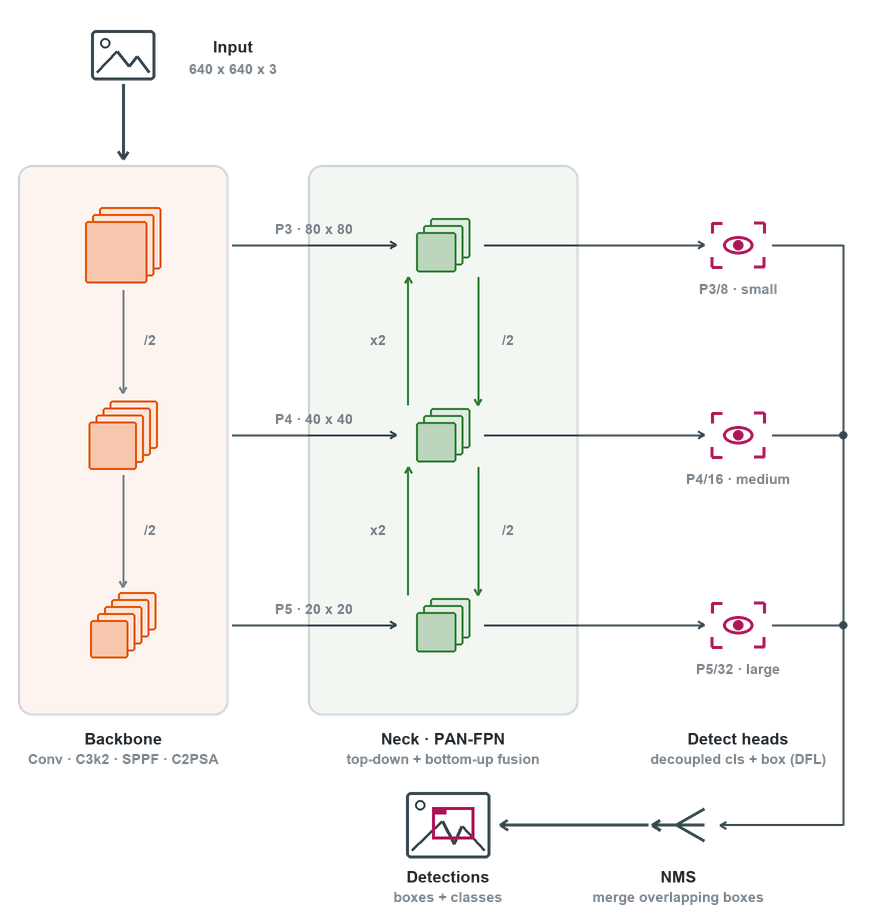
\includegraphics[width=\textwidth]{./figures/yolo11_architecture_abstract.png}
    \caption{Internal architecture of the YOLO11 detector.}
    \label{fig:YOLO11}
\end{figure}

Reading Figure~\ref{fig:YOLO11} top to bottom, the $640\times640$ input passes through Conv, C3k2, SPPF, and C2PSA backbone blocks, producing P3, P4, and P5 feature maps at strides 8, 16, and 32 ($80\times80$, $40\times40$, and $20\times20$). C3k2 provides convolutional feature aggregation, SPPF combines pooled context, and C2PSA adds partial self-attention. The PAN/FPN neck combines features through top-down upsampling and bottom-up downsampling. At each scale, separate anchor-free head branches predict classes and box offsets, with distribution-focal training for box regression. Non-maximum suppression removes overlapping candidate detections before the highest-confidence box is selected.

\subsection{Why YOLO11}
YOLO11 was chosen for architectural and practical reasons made concrete by Figure~\ref{fig:YOLO11}. Its C2PSA partial self-attention and multi-scale feature fusion provide context for localizing waste under varied backgrounds; its C3k2 blocks and anchor-free decoupled head support a compact detector at the ``s'' scale; and the Ultralytics tooling provides a consistent path for training, validation-mAP checkpointing, and inference.

The choice is also supported by the detector benchmark in the Results chapter (Table~\ref{tab:det_compare}). YOLO11s attains the highest F1 ($0.9869$) and precision ($0.9886$), an mAP@50 of $0.9906$, and an mAP@50:95 of $0.8458$, with an inference time of $9.15$~ms per image. YOLOv12s achieves higher mAP@50:95 ($0.8566$) at $12.81$~ms, while YOLOv10s is slightly faster ($9.03$~ms). The choice of YOLO11s therefore balances localization accuracy and inference time. The separate evaluation of the pipeline detector on 221 test views obtains mAP@50 $0.9922$ and mAP@50:95 $0.8534$.

\subsection{Detector Training and Inference}
The detector is trained with the Ultralytics recipe (input $640\times640$, mosaic and colour augmentation, box, class, and distribution-focal losses) on the same training items used for the classifier, and the best checkpoint is chosen by validation mAP. At inference, detect\_top\_crop keeps only the highest-confidence box per image and passes the padded crop to the classifier. The detector is evaluated by mean Average Precision, and the full pipeline is additionally evaluated end-to-end against an oracle (ground-truth) crop to quantify the localization cost separately from the classification cost.

\section{Proposed Multi-Task Network}
The cropped object is encoded by one shared backbone into a feature vector that is consumed by four task-specific heads. The architecture, implemented as MultiTaskNet, uses the backbone shown in Figure~\ref{fig:ConvNext}.

\subsection{Backbone Candidates}
Nine backbones spanning convolutional and transformer families were evaluated as the shared trunk. Table~\ref{tab:backbone_candidates} lists them together with their family, approximate parameter count, and pretraining. The set spans lightweight mobile CNNs (EfficientNet-B0, MobileNetV3-Large), a deep residual CNN (ResNet50), the modernized ConvNeXt family in two capacities (ConvNeXt-T, ConvNeXt-S), and four vision transformers of different scales and pretraining objectives (DINOv2 ViT-S and ViT-B, register-token DINOv2 ViT-S, and SigLIP ViT-B). The baseline recipe is given in Table~\ref{tab:hyper}; the larger and register-token transformers use the specialised small-data recipe described below. A four-backbone feature-fusion ensemble is also evaluated (Section~\ref{sec:fusion}).

\begin{table}[!ht]
\centering
\caption{Backbone candidates evaluated as the shared trunk.}
\label{tab:backbone_candidates}
\begin{tabularx}{\linewidth}{@{}l l c Y@{}}
\toprule
\textbf{Backbone} & \textbf{Family} & \textbf{Params (M)} & \textbf{Pretraining} \\
\midrule
EfficientNet-B0     & CNN (mobile)        & 5.3  & ImageNet-1k \\
MobileNetV3-Large   & CNN (mobile)        & 5.5  & ImageNet-1k \\
ResNet50            & CNN (residual)      & 25.6 & ImageNet-1k \\
ConvNeXt-T          & CNN (modernized)    & 28.6 & ImageNet-1k \\
\textbf{ConvNeXt-S} & CNN (modernized)    & 50.2 & ImageNet-22k, then ImageNet-1k \\
DINOv2 ViT-S/14     & Transformer         & 22.1 & self-supervised \\
DINOv2 ViT-S/14 +reg & Transformer        & 22.1 & self-supervised  \\
DINOv2 ViT-B/14     & Transformer         & 86.6 & self-supervised \\
SigLIP ViT-B/16     & Transformer         & 85.8 & vision-language \\
\bottomrule
\end{tabularx}
\end{table}

\subsection{ConvNeXt-S Architecture}
The selected backbone is ConvNeXt-S pretrained on ImageNet-22k and subsequently fine-tuned on ImageNet-1k \cite{convnext}, whose structure is shown in Figure~\ref{fig:ConvNext}. ConvNeXt is a purely convolutional network that adopts several design choices from vision transformers while retaining the inductive bias of convolution.

\begin{figure}[!ht]
    \centering
    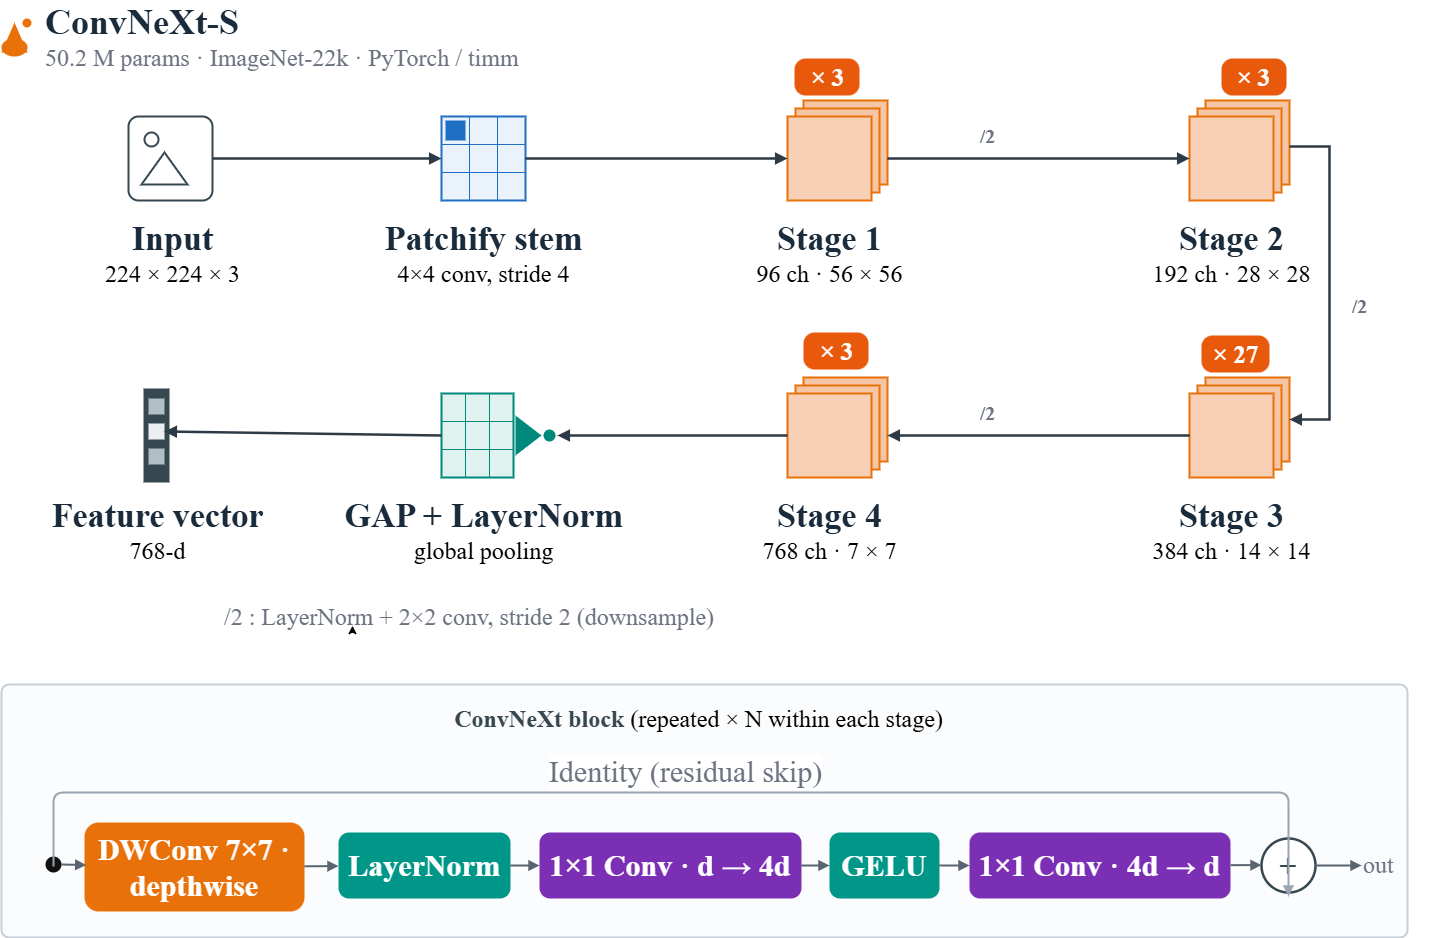
\includegraphics[height=12.5cm,width=\textwidth]{./figures/convnext_s_architecture_abstract.png}
    \caption{Internal architecture of the ConvNeXt-S backbone.}
    \label{fig:ConvNext}
\end{figure}

Figure~\ref{fig:ConvNext} shows the four elements that define ConvNeXt-S. The patchify stem uses a $4\times4$ stride-4 convolution, analogous to transformer tokenization. The four stages follow the depth ratio $[3,3,27,3]$ with channel widths $[96,192,384,768]$, joined by downsampling layers (layer normalization plus a $2\times2$ stride-2 convolution) that halve the resolution and double the width. Each ConvNeXt block, drawn in the inset, uses a large $7\times7$ depthwise convolution, followed by an inverted bottleneck (layer normalization, a $1\times1$ expansion to four times the width, GELU, and a $1\times1$ projection back) and an identity residual connection. The final global average pooling and layer normalization produce the $768$-dimensional feature that all four heads consume. Parameter counts in Table~\ref{tab:backbone_candidates} are approximate architecture sizes.

\subsection{Why ConvNeXt-S}
ConvNeXt-S was selected for reasons that combine architecture and evidence. Its large-kernel depthwise convolutions provide a wide receptive field, while the deeper third stage and ImageNet pretraining supply transferable features for material discrimination. Empirically, ConvNeXt-S obtained the highest single-backbone material macro-F1 ($0.8395$) on the 50-item test set, ahead of DINOv2 ViT-B ($0.8181$). Material is central to the routing matrix and material-specific overrides. DINOv2 ViT-B performs better on route macro-F1 ($0.8174$ against $0.7396$), threat QWK ($0.8390$ against $0.8261$), and raw material calibration (ECE $0.0713$ against $0.1102$), while carrying a larger nominal architecture ($86.6$M against $50.2$M). The selection therefore prioritizes material performance and a single shared convolutional backbone, with cross-head reconciliation and safety rules applied at the decision layer. The full per-head comparison is reported in the Results chapter (Table~\ref{tab:backbones}).

\subsection{Vision-Transformer Fine-Tuning and Feature Fusion}
\label{sec:fusion}
The larger and register-token vision transformers are trained with a specialised small-data recipe: layer-wise learning-rate decay gives earlier blocks progressively smaller learning rates; a linear-probe-then-fine-tune schedule first warms up the task heads with the backbone frozen and then unfreezes the backbone at a low rate; selected early blocks can remain frozen; and stochastic depth provides regularisation. Plain DINOv2 ViT-S uses the baseline recipe, so the plain and register-token variants compare both model representation and fine-tuning strategy.

Separately, a feature-fusion model concatenates the pooled features of fine-tuned ConvNeXt-S, ConvNeXt-T, ResNet50, and DINOv2 ViT-B, passes them through a small fusion network, and feeds the same four heads, with member backbones frozen so only the fusion and heads train. Fusing these domain-adapted backbones yields material macro-F1 $0.8395$, material ECE $0.0584$, and threat QWK $0.8571$. The model is reported alongside the single backbones in the Results chapter.

\subsection{Task Heads}
Each head is the same small module (Head): a linear projection to a $256$-unit hidden layer, batch normalization, a GELU non-linearity, dropout at rate $0.2$, and a final linear layer to the task output size. The material head outputs $10$ logits, the condition head a single logit, the route head $4$ logits, and the threat head $K-1=3$ logits in the CORN ordinal parameterization. The forward pass returns all four outputs from one shared feature. Figure~\ref{fig:detclf_example} traces the two-stage inference on item~106. YOLO11 localizes the broken glass with box confidence $0.91$; the highest-confidence box is cropped to $224\times224$ and encoded by ConvNeXt-S, whose heads emit, after averaging the item's three views, material glass ($0.99$ confidence), condition Poor ($P(\text{Poor})$ rounded to $1.00$), route Special ($0.87$ confidence), and threat level~3. These are the raw head predictions before the decision layer, which confirms Special through the broken-glass rule and threat backstop (Figure~\ref{fig:Decision}).

\begin{figure}[!ht]
    \centering
    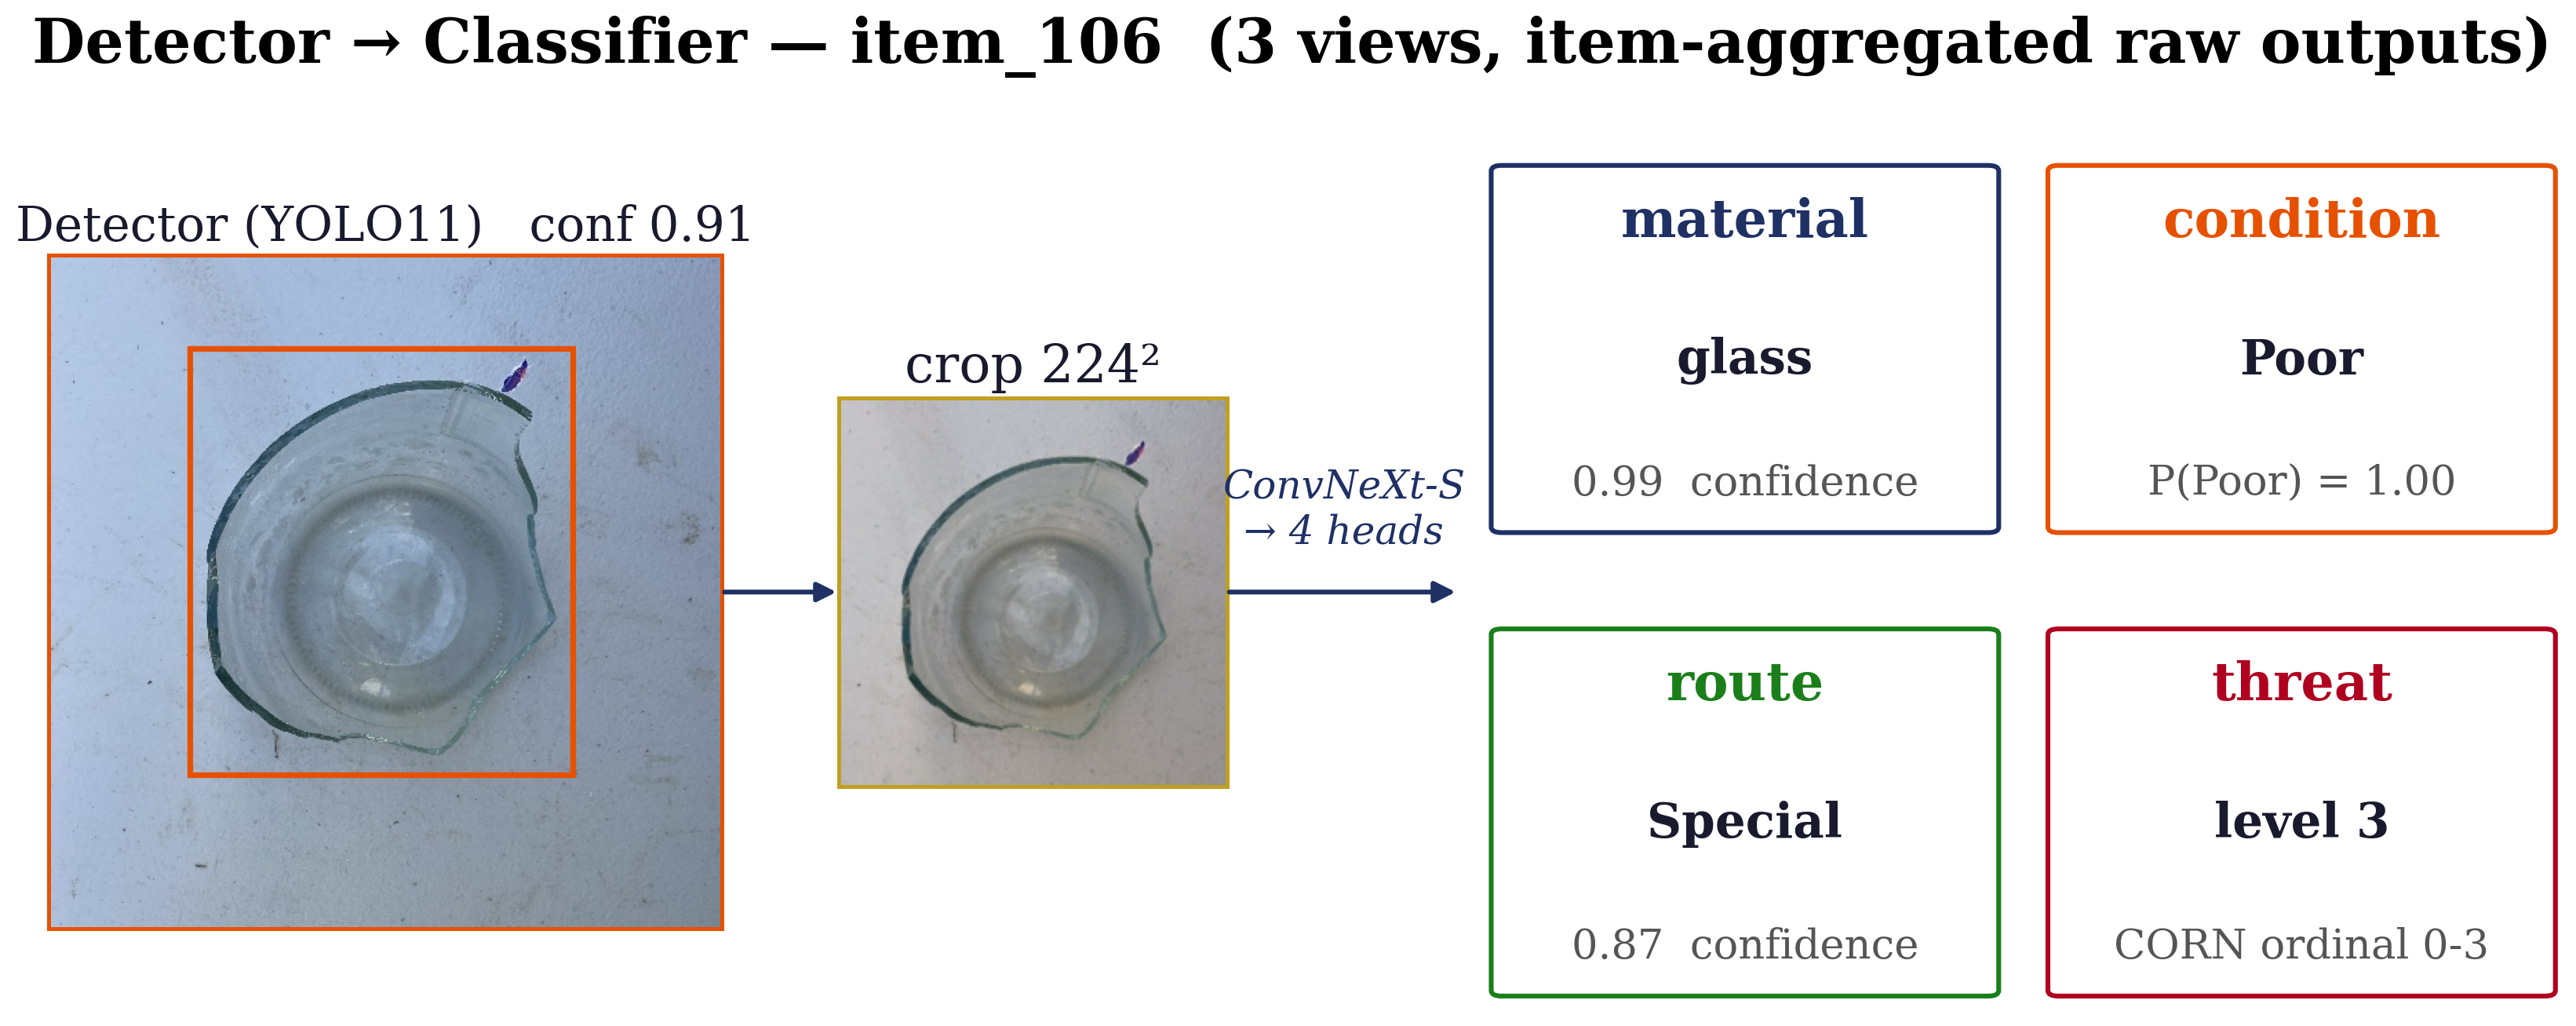
\includegraphics[height=5cm,width=\textwidth]{./figures/fig3_detector_classifier_transparent.png}
    \caption{The full detect $\rightarrow$ classify inference on one real item (item~106).}
    \label{fig:detclf_example}
\end{figure}

\section{Loss Functions}
The four heads are trained jointly, each with a task-appropriate loss.

\textbf{Material (class-balanced focal loss).} The material head uses the focal loss \cite{focal} (focal\_loss), which down-weights easy examples, with per-class balancing weights $\alpha_c$ obtained from cb\_weights (normalized inverse training-image counts $1/(n_c+1)$):
\begin{equation}
\mathcal{L}_{\text{mat}} = -\,\alpha_{c}\,(1-p_t)^{\gamma}\,\log(p_t),
\end{equation}
where $p_t$ is the predicted probability of the true class and $\gamma=2$ is the focusing parameter.

\textbf{Condition (binary cross-entropy).}
\begin{equation}
\mathcal{L}_{\text{cond}} = -\big[y\log\sigma(z) + (1-y)\log(1-\sigma(z))\big].
\end{equation}

\textbf{Route (weighted cross-entropy with label smoothing).} The route head uses cross-entropy with class weights $w_r$ (from cb\_weights, to counter the dominance of Special and scarcity of Reuse) and label smoothing:
\begin{equation}
\mathcal{L}_{\text{route}} = -\sum_{k} w_{k}\,\tilde{y}_k \log p_k .
\end{equation}

\textbf{Threat (CORN ordinal loss).} Because threat is ordered, the threat head uses the rank-consistent CORN formulation \cite{corn} (corn\_loss), which decomposes the $K=4$-level ordinal task into $K-1=3$ conditional binary problems. Products of the conditional sigmoid probabilities produce non-increasing cumulative probabilities. Head metrics decode the level by counting cumulative probabilities above $0.5$, whereas routing uses the most probable threat class.

\textbf{Aggregation.} The total objective is a weighted sum of the four losses with fixed weights LOSS\_W: material $1.0$, condition $0.5$, route $1.0$, and threat $1.0$. An optional uncertainty-based weighting is available but left off in these experiments.

\section{Training Procedure}
The baseline backbones are trained by a single routine (train\_backbone $\rightarrow$ \_fit) under the recipe in Table~\ref{tab:hyper}. The procedure is:
\begin{enumerate}
    \item \textbf{Parameter groups.} Parameters are split into a backbone group and a head group, optimized by AdamW with a small backbone learning rate ($3\times10^{-5}$) and a larger head rate ($3\times10^{-4}$), so the pretrained features are preserved while the new heads adapt quickly.
    \item \textbf{Schedule.} A cosine learning-rate schedule with a two-epoch linear warmup is applied per step.
    \item \textbf{Mixed precision.} Forward and backward passes run under automatic mixed precision (GradScaler); gradients are clipped to a norm of $1.0$ for stability.
    \item \textbf{Weight averaging.} An exponential moving average of the weights (ModelEmaV2, decay warmed up to $0.998$) is maintained and used for validation and checkpoint selection.
    \item \textbf{Model selection.} After each epoch the EMA model is evaluated on the validation split, and a composite score, $0.4\,(\text{route F1}) + 0.4\,(\text{threat QWK}) + 0.2\,(\text{material F1})$, is computed; the best-scoring checkpoint is retained.
    \item \textbf{Early stopping.} Training stops if the validation score does not improve for six consecutive epochs (a maximum of $24$).
    \item \textbf{Test-time augmentation.} At evaluation, logits are averaged over the image and its horizontal flip before item aggregation. A separate augmentation experiment averages four deterministic variants: the base image, horizontal flip, zoom, and zoom with horizontal flip.
\end{enumerate}
The specialised transformer procedure retains these losses, EMA, and validation score while using probing and layer-wise fine-tuning as described in Section~\ref{sec:fusion}.

\begin{table}[!ht]
\centering
\caption{Training hyperparameters.}
\label{tab:hyper}
\begin{tabularx}{0.92\linewidth}{@{}l Y@{}}
\toprule
\textbf{Hyperparameter} & \textbf{Value} \\
\midrule
Input resolution & $224 \times 224$ \\
Batch size & 32 \\
Optimizer & AdamW \\
Learning rate (heads / backbone) & $3\times10^{-4}$ / $3\times10^{-5}$ \\
Schedule & cosine with 2-epoch warmup \\
Max epochs & 24 (early stopping, patience 6) \\
Weight decay & $1\times10^{-3}$ \\
EMA decay & 0.998 \\
Label smoothing (route) & 0.05 \\
Class imbalance & class-balanced focal + inverse-frequency sampling \\
Random seed & 42 \\
\bottomrule
\end{tabularx}
\end{table}

\section{Calibration}
Modern networks can be over-confident, so temperature scaling is evaluated after training \cite{guo2017}. A positive scalar $T$ fitted on the validation split rescales the material and route logits, $\hat{p}=\mathrm{softmax}(z/T)$, while condition uses $\sigma(z/T)$ and threat uses the corresponding CORN probabilities. Separate fitters are used for the head types: fit\_T\_softmax (material and route), fit\_T\_binary (condition), and fit\_T\_corn (threat). A positive scalar preserves the softmax arg-max and the condition threshold at $0.5$; however, temperature scaling can change the cumulative CORN prediction, so threat metrics are recomputed after calibration. The guarded scalar procedure in Figure~\ref{fig:Flowchart} retains a fitted temperature only when it improves validation ECE, otherwise using $T=1$.

The calibration experiment uses a three-backbone fusion of ConvNeXt-S, ResNet50, and DINOv2 ViT-S. Material, route, and condition temperatures are $1.0000$, $0.9965$, and $3.5193$, respectively; the threat head uses separate cut-point temperatures $[0.5000,2.6435,3.3070]$, rather than the shared scalar illustrated in the flowchart. Test ECE changes from $0.1143$ to $0.1143$ for material, $0.1894$ to $0.1888$ for route, $0.2191$ to $0.1120$ for condition, and $0.0871$ to $0.1015$ for threat. Calibration therefore substantially improves condition confidence, while the threat result illustrates the need to assess calibration separately for each head. Calibration quality is reported with ECE and reliability diagrams. Calibrated confidences can support the abstention gate, while the paired end-to-end evaluation uses unscaled probabilities.

\section{Decision Layer}
The four head outputs are fused by the confidence-aware decide engine shown in Figure~\ref{fig:Decision}. The earlier pooled policy evaluation uses apply\_policy, which omits learned-route and threat-prior reconciliation and refers remaining low-material-confidence items for review. The diagrammed engine is used for the paired end-to-end evaluation.

\begin{figure}[!ht]
    \centering
    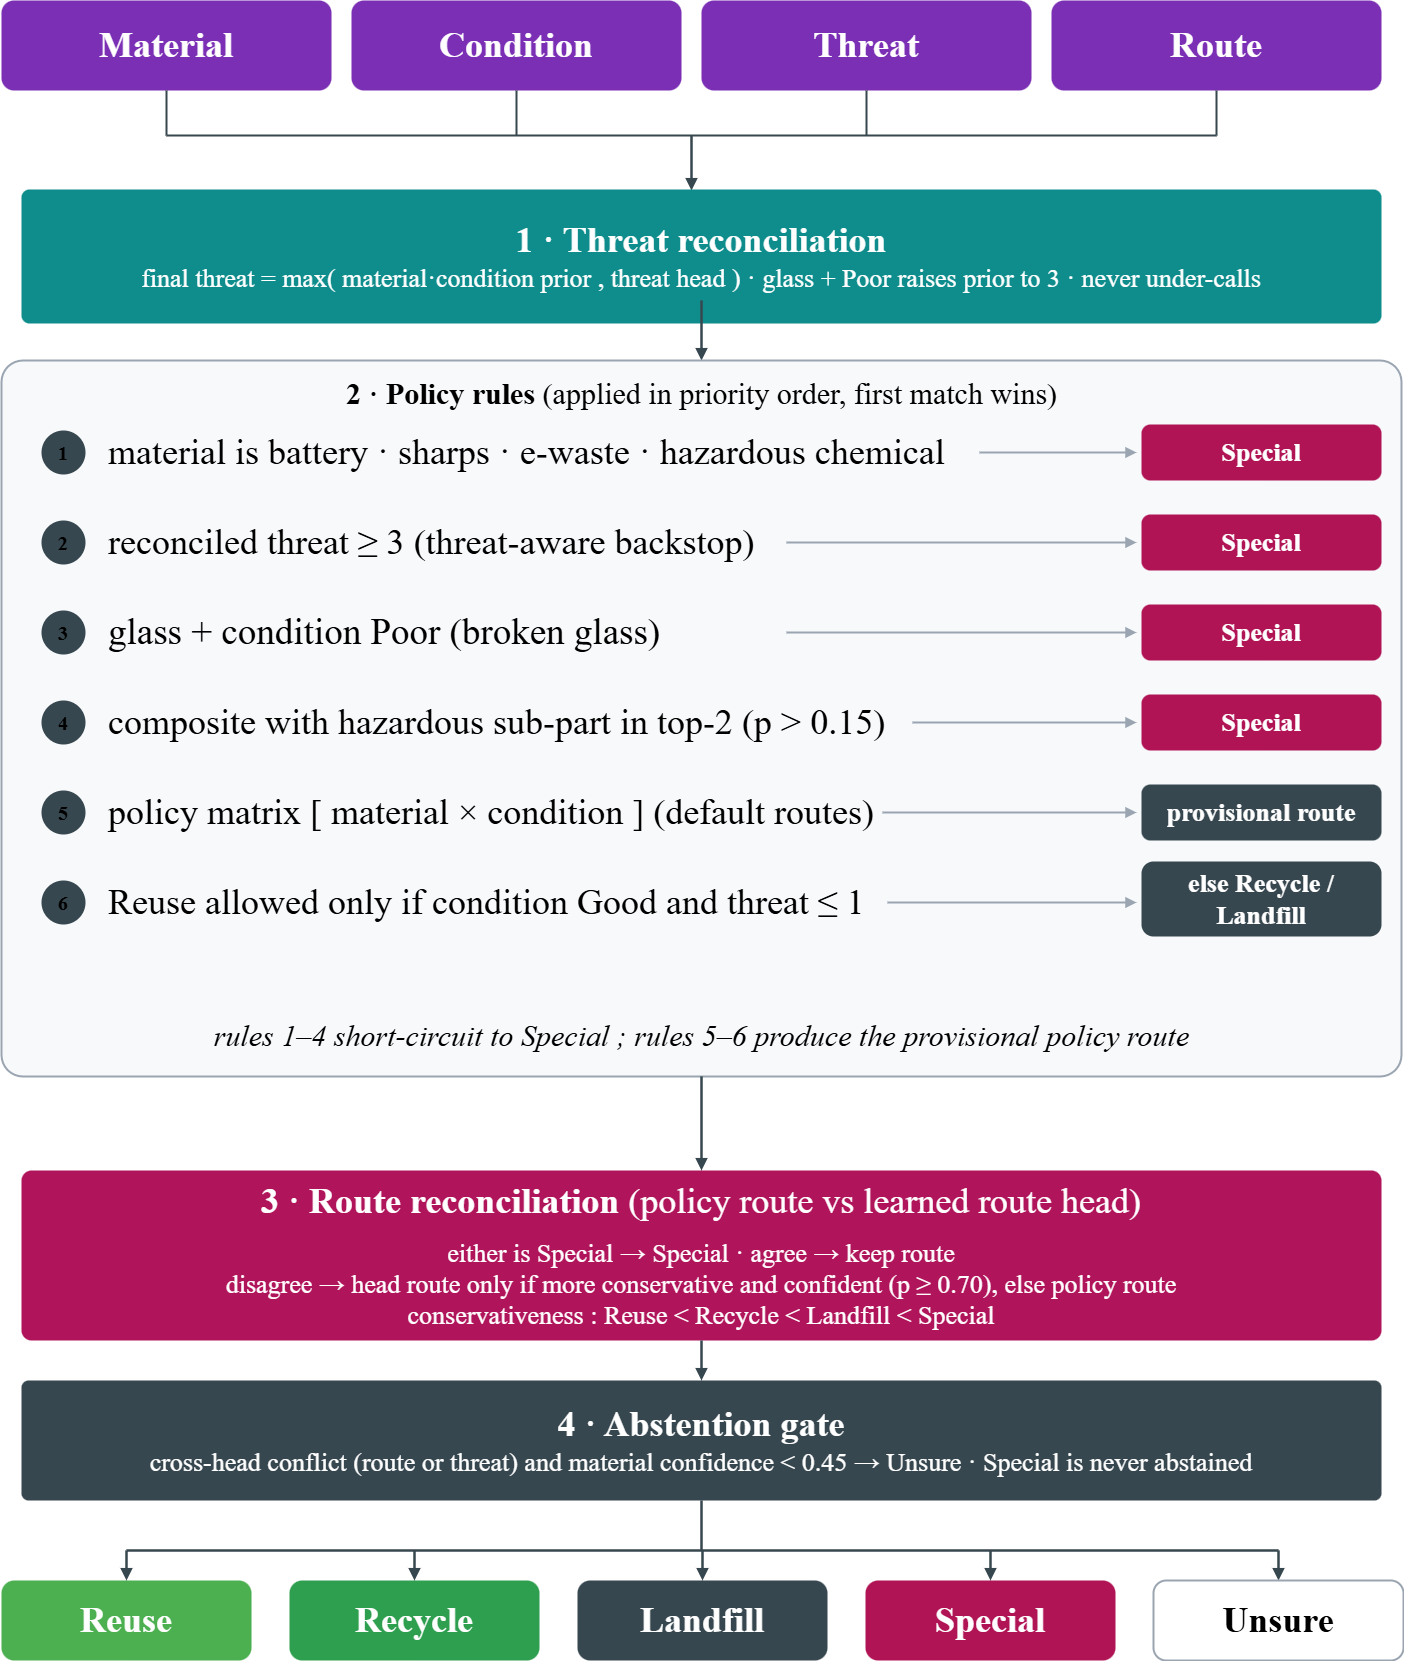
\includegraphics[height=16.5cm,width=\textwidth]{./figures/decision_layer.png}
    \caption{Stages of the decision layer.}
    \label{fig:Decision}
\end{figure}

Following the stages of Figure~\ref{fig:Decision}, the four item-level head outputs enter at the top. Stage~1 reconciles threat by taking the maximum of the material-and-condition prior and the most probable threat-head class; glass in Poor condition raises the prior to 3. Stage~2 applies the priority-ordered policy rules: force-Special materials, the threat backstop, glass in Poor condition, and a composite with a hazardous material among its top two predictions (probability $>0.15$), followed by the material$\times$condition matrix and Reuse gate. Reuse is allowed only if condition is Good and threat $\le1$; a reconciled threat $\ge3$ forces Special independently of the material label. Stage~3 reconciles the policy route with the learned route head: Special from either estimate is retained, agreement preserves the route, and a disagreeing learned route is accepted only if it is more conservative and its confidence is at least $0.70$. Stage~4 abstains (``Unsure'') only when a route or threat conflict accompanies material confidence below $0.45$, and Special is never abstained. The outputs are the final route, reconciled threat, a confidence value (the minimum of material, threat, and route-head confidences), and a rule-trace explanation. Decision quality is summarized by hazard-weighted cost, coverage, and hazard recall. Hazard-handling recall counts ground-truth Special items either routed to Special or referred as Unsure; strict Special-routing recall counts only those routed to Special. Abstentions are excluded from accumulated cost and reported through coverage.

\section{Evaluation Protocol}
Predictions are produced and scored at the item level: evaluate\_logits collects per-image head logits, aggregate\_by\_item averages the logits of an item's views, and item\_metrics/full\_report compute per-head metrics (material accuracy and macro-F1, route macro-F1, condition AUROC, threat QWK and MAE, and per-class scores). Two protocols are used: a single held-out split of 50 items with 221 test views, and pooled out-of-fold evaluation covering 457 items and 1{,}961 views. Out-of-fold splitting is performed over items, stratified by material, with an internal validation subset for checkpoint selection. The 457-item evaluation precedes the expansion to the 485-item dataset described above. Bootstrap $95\%$ confidence intervals are computed from 5{,}000 item resamples. The detector is scored by image-level precision, recall, and mean Average Precision; oracle and detector crops are compared to measure the end-to-end localization effect. External generalization is assessed on TrashNet and TACO using the applicable material mappings and detection annotations.

\section{Conclusion}
This chapter detailed the complete methodology: the purpose-built real-world dataset and its leakage-controlled item-level split, the per-image preprocessing chain, the two-stage detect-then-classify architecture, the choice and internal structure of the YOLO11 detector and the ConvNeXt-S backbone, the four task heads, the loss functions, the training procedure, per-head calibration, the regulation-grounded decision layer with its safety backstop, and the item-level evaluation protocol. Each step was tied to the concrete operation that implements it, and each figure was described at the point where it was introduced. The next chapter evaluates the resulting system.
